% Options for packages loaded elsewhere
\PassOptionsToPackage{unicode}{hyperref}
\PassOptionsToPackage{hyphens}{url}
\PassOptionsToPackage{dvipsnames,svgnames,x11names}{xcolor}
%
\documentclass[
  letterpaper,
  DIV=11,
  numbers=noendperiod]{scrartcl}

\usepackage{amsmath,amssymb}
\usepackage{lmodern}
\usepackage{iftex}
\ifPDFTeX
  \usepackage[T1]{fontenc}
  \usepackage[utf8]{inputenc}
  \usepackage{textcomp} % provide euro and other symbols
\else % if luatex or xetex
  \usepackage{unicode-math}
  \defaultfontfeatures{Scale=MatchLowercase}
  \defaultfontfeatures[\rmfamily]{Ligatures=TeX,Scale=1}
\fi
% Use upquote if available, for straight quotes in verbatim environments
\IfFileExists{upquote.sty}{\usepackage{upquote}}{}
\IfFileExists{microtype.sty}{% use microtype if available
  \usepackage[]{microtype}
  \UseMicrotypeSet[protrusion]{basicmath} % disable protrusion for tt fonts
}{}
\makeatletter
\@ifundefined{KOMAClassName}{% if non-KOMA class
  \IfFileExists{parskip.sty}{%
    \usepackage{parskip}
  }{% else
    \setlength{\parindent}{0pt}
    \setlength{\parskip}{6pt plus 2pt minus 1pt}}
}{% if KOMA class
  \KOMAoptions{parskip=half}}
\makeatother
\usepackage{xcolor}
\setlength{\emergencystretch}{3em} % prevent overfull lines
\setcounter{secnumdepth}{-\maxdimen} % remove section numbering
% Make \paragraph and \subparagraph free-standing
\ifx\paragraph\undefined\else
  \let\oldparagraph\paragraph
  \renewcommand{\paragraph}[1]{\oldparagraph{#1}\mbox{}}
\fi
\ifx\subparagraph\undefined\else
  \let\oldsubparagraph\subparagraph
  \renewcommand{\subparagraph}[1]{\oldsubparagraph{#1}\mbox{}}
\fi

\usepackage{color}
\usepackage{fancyvrb}
\newcommand{\VerbBar}{|}
\newcommand{\VERB}{\Verb[commandchars=\\\{\}]}
\DefineVerbatimEnvironment{Highlighting}{Verbatim}{commandchars=\\\{\}}
% Add ',fontsize=\small' for more characters per line
\usepackage{framed}
\definecolor{shadecolor}{RGB}{241,243,245}
\newenvironment{Shaded}{\begin{snugshade}}{\end{snugshade}}
\newcommand{\AlertTok}[1]{\textcolor[rgb]{0.68,0.00,0.00}{#1}}
\newcommand{\AnnotationTok}[1]{\textcolor[rgb]{0.37,0.37,0.37}{#1}}
\newcommand{\AttributeTok}[1]{\textcolor[rgb]{0.40,0.45,0.13}{#1}}
\newcommand{\BaseNTok}[1]{\textcolor[rgb]{0.68,0.00,0.00}{#1}}
\newcommand{\BuiltInTok}[1]{\textcolor[rgb]{0.00,0.23,0.31}{#1}}
\newcommand{\CharTok}[1]{\textcolor[rgb]{0.13,0.47,0.30}{#1}}
\newcommand{\CommentTok}[1]{\textcolor[rgb]{0.37,0.37,0.37}{#1}}
\newcommand{\CommentVarTok}[1]{\textcolor[rgb]{0.37,0.37,0.37}{\textit{#1}}}
\newcommand{\ConstantTok}[1]{\textcolor[rgb]{0.56,0.35,0.01}{#1}}
\newcommand{\ControlFlowTok}[1]{\textcolor[rgb]{0.00,0.23,0.31}{#1}}
\newcommand{\DataTypeTok}[1]{\textcolor[rgb]{0.68,0.00,0.00}{#1}}
\newcommand{\DecValTok}[1]{\textcolor[rgb]{0.68,0.00,0.00}{#1}}
\newcommand{\DocumentationTok}[1]{\textcolor[rgb]{0.37,0.37,0.37}{\textit{#1}}}
\newcommand{\ErrorTok}[1]{\textcolor[rgb]{0.68,0.00,0.00}{#1}}
\newcommand{\ExtensionTok}[1]{\textcolor[rgb]{0.00,0.23,0.31}{#1}}
\newcommand{\FloatTok}[1]{\textcolor[rgb]{0.68,0.00,0.00}{#1}}
\newcommand{\FunctionTok}[1]{\textcolor[rgb]{0.28,0.35,0.67}{#1}}
\newcommand{\ImportTok}[1]{\textcolor[rgb]{0.00,0.46,0.62}{#1}}
\newcommand{\InformationTok}[1]{\textcolor[rgb]{0.37,0.37,0.37}{#1}}
\newcommand{\KeywordTok}[1]{\textcolor[rgb]{0.00,0.23,0.31}{#1}}
\newcommand{\NormalTok}[1]{\textcolor[rgb]{0.00,0.23,0.31}{#1}}
\newcommand{\OperatorTok}[1]{\textcolor[rgb]{0.37,0.37,0.37}{#1}}
\newcommand{\OtherTok}[1]{\textcolor[rgb]{0.00,0.23,0.31}{#1}}
\newcommand{\PreprocessorTok}[1]{\textcolor[rgb]{0.68,0.00,0.00}{#1}}
\newcommand{\RegionMarkerTok}[1]{\textcolor[rgb]{0.00,0.23,0.31}{#1}}
\newcommand{\SpecialCharTok}[1]{\textcolor[rgb]{0.37,0.37,0.37}{#1}}
\newcommand{\SpecialStringTok}[1]{\textcolor[rgb]{0.13,0.47,0.30}{#1}}
\newcommand{\StringTok}[1]{\textcolor[rgb]{0.13,0.47,0.30}{#1}}
\newcommand{\VariableTok}[1]{\textcolor[rgb]{0.07,0.07,0.07}{#1}}
\newcommand{\VerbatimStringTok}[1]{\textcolor[rgb]{0.13,0.47,0.30}{#1}}
\newcommand{\WarningTok}[1]{\textcolor[rgb]{0.37,0.37,0.37}{\textit{#1}}}

\providecommand{\tightlist}{%
  \setlength{\itemsep}{0pt}\setlength{\parskip}{0pt}}\usepackage{longtable,booktabs,array}
\usepackage{calc} % for calculating minipage widths
% Correct order of tables after \paragraph or \subparagraph
\usepackage{etoolbox}
\makeatletter
\patchcmd\longtable{\par}{\if@noskipsec\mbox{}\fi\par}{}{}
\makeatother
% Allow footnotes in longtable head/foot
\IfFileExists{footnotehyper.sty}{\usepackage{footnotehyper}}{\usepackage{footnote}}
\makesavenoteenv{longtable}
\usepackage{graphicx}
\makeatletter
\def\maxwidth{\ifdim\Gin@nat@width>\linewidth\linewidth\else\Gin@nat@width\fi}
\def\maxheight{\ifdim\Gin@nat@height>\textheight\textheight\else\Gin@nat@height\fi}
\makeatother
% Scale images if necessary, so that they will not overflow the page
% margins by default, and it is still possible to overwrite the defaults
% using explicit options in \includegraphics[width, height, ...]{}
\setkeys{Gin}{width=\maxwidth,height=\maxheight,keepaspectratio}
% Set default figure placement to htbp
\makeatletter
\def\fps@figure{htbp}
\makeatother

\KOMAoption{captions}{tableheading}
\makeatletter
\makeatother
\makeatletter
\makeatother
\makeatletter
\@ifpackageloaded{caption}{}{\usepackage{caption}}
\AtBeginDocument{%
\ifdefined\contentsname
  \renewcommand*\contentsname{Table of contents}
\else
  \newcommand\contentsname{Table of contents}
\fi
\ifdefined\listfigurename
  \renewcommand*\listfigurename{List of Figures}
\else
  \newcommand\listfigurename{List of Figures}
\fi
\ifdefined\listtablename
  \renewcommand*\listtablename{List of Tables}
\else
  \newcommand\listtablename{List of Tables}
\fi
\ifdefined\figurename
  \renewcommand*\figurename{Figure}
\else
  \newcommand\figurename{Figure}
\fi
\ifdefined\tablename
  \renewcommand*\tablename{Table}
\else
  \newcommand\tablename{Table}
\fi
}
\@ifpackageloaded{float}{}{\usepackage{float}}
\floatstyle{ruled}
\@ifundefined{c@chapter}{\newfloat{codelisting}{h}{lop}}{\newfloat{codelisting}{h}{lop}[chapter]}
\floatname{codelisting}{Listing}
\newcommand*\listoflistings{\listof{codelisting}{List of Listings}}
\makeatother
\makeatletter
\@ifpackageloaded{caption}{}{\usepackage{caption}}
\@ifpackageloaded{subcaption}{}{\usepackage{subcaption}}
\makeatother
\makeatletter
\@ifpackageloaded{tcolorbox}{}{\usepackage[many]{tcolorbox}}
\makeatother
\makeatletter
\@ifundefined{shadecolor}{\definecolor{shadecolor}{rgb}{.97, .97, .97}}
\makeatother
\makeatletter
\makeatother
\ifLuaTeX
  \usepackage{selnolig}  % disable illegal ligatures
\fi
\IfFileExists{bookmark.sty}{\usepackage{bookmark}}{\usepackage{hyperref}}
\IfFileExists{xurl.sty}{\usepackage{xurl}}{} % add URL line breaks if available
\urlstyle{same} % disable monospaced font for URLs
\hypersetup{
  pdftitle={git\_tutorial\_notes},
  colorlinks=true,
  linkcolor={blue},
  filecolor={Maroon},
  citecolor={Blue},
  urlcolor={Blue},
  pdfcreator={LaTeX via pandoc}}

\title{git\_tutorial\_notes}
\author{}
\date{}

\begin{document}
\maketitle
\ifdefined\Shaded\renewenvironment{Shaded}{\begin{tcolorbox}[interior hidden, enhanced, frame hidden, boxrule=0pt, breakable, sharp corners, borderline west={3pt}{0pt}{shadecolor}]}{\end{tcolorbox}}\fi

\hypertarget{getting-started-with-github-git-and-r-studio.}{%
\section{Getting started with github, git and
R-studio.}\label{getting-started-with-github-git-and-r-studio.}}

\hypertarget{creating-a-github-account}{%
\subsubsection{Creating a github
account}\label{creating-a-github-account}}

Go to the github \href{http://github.com}{website}

\begin{figure}

{\centering 
\includegraphics{figures/1.PNG}

}

\caption{Github website}

\end{figure}

and signup with your email and password.

\begin{figure}

{\centering 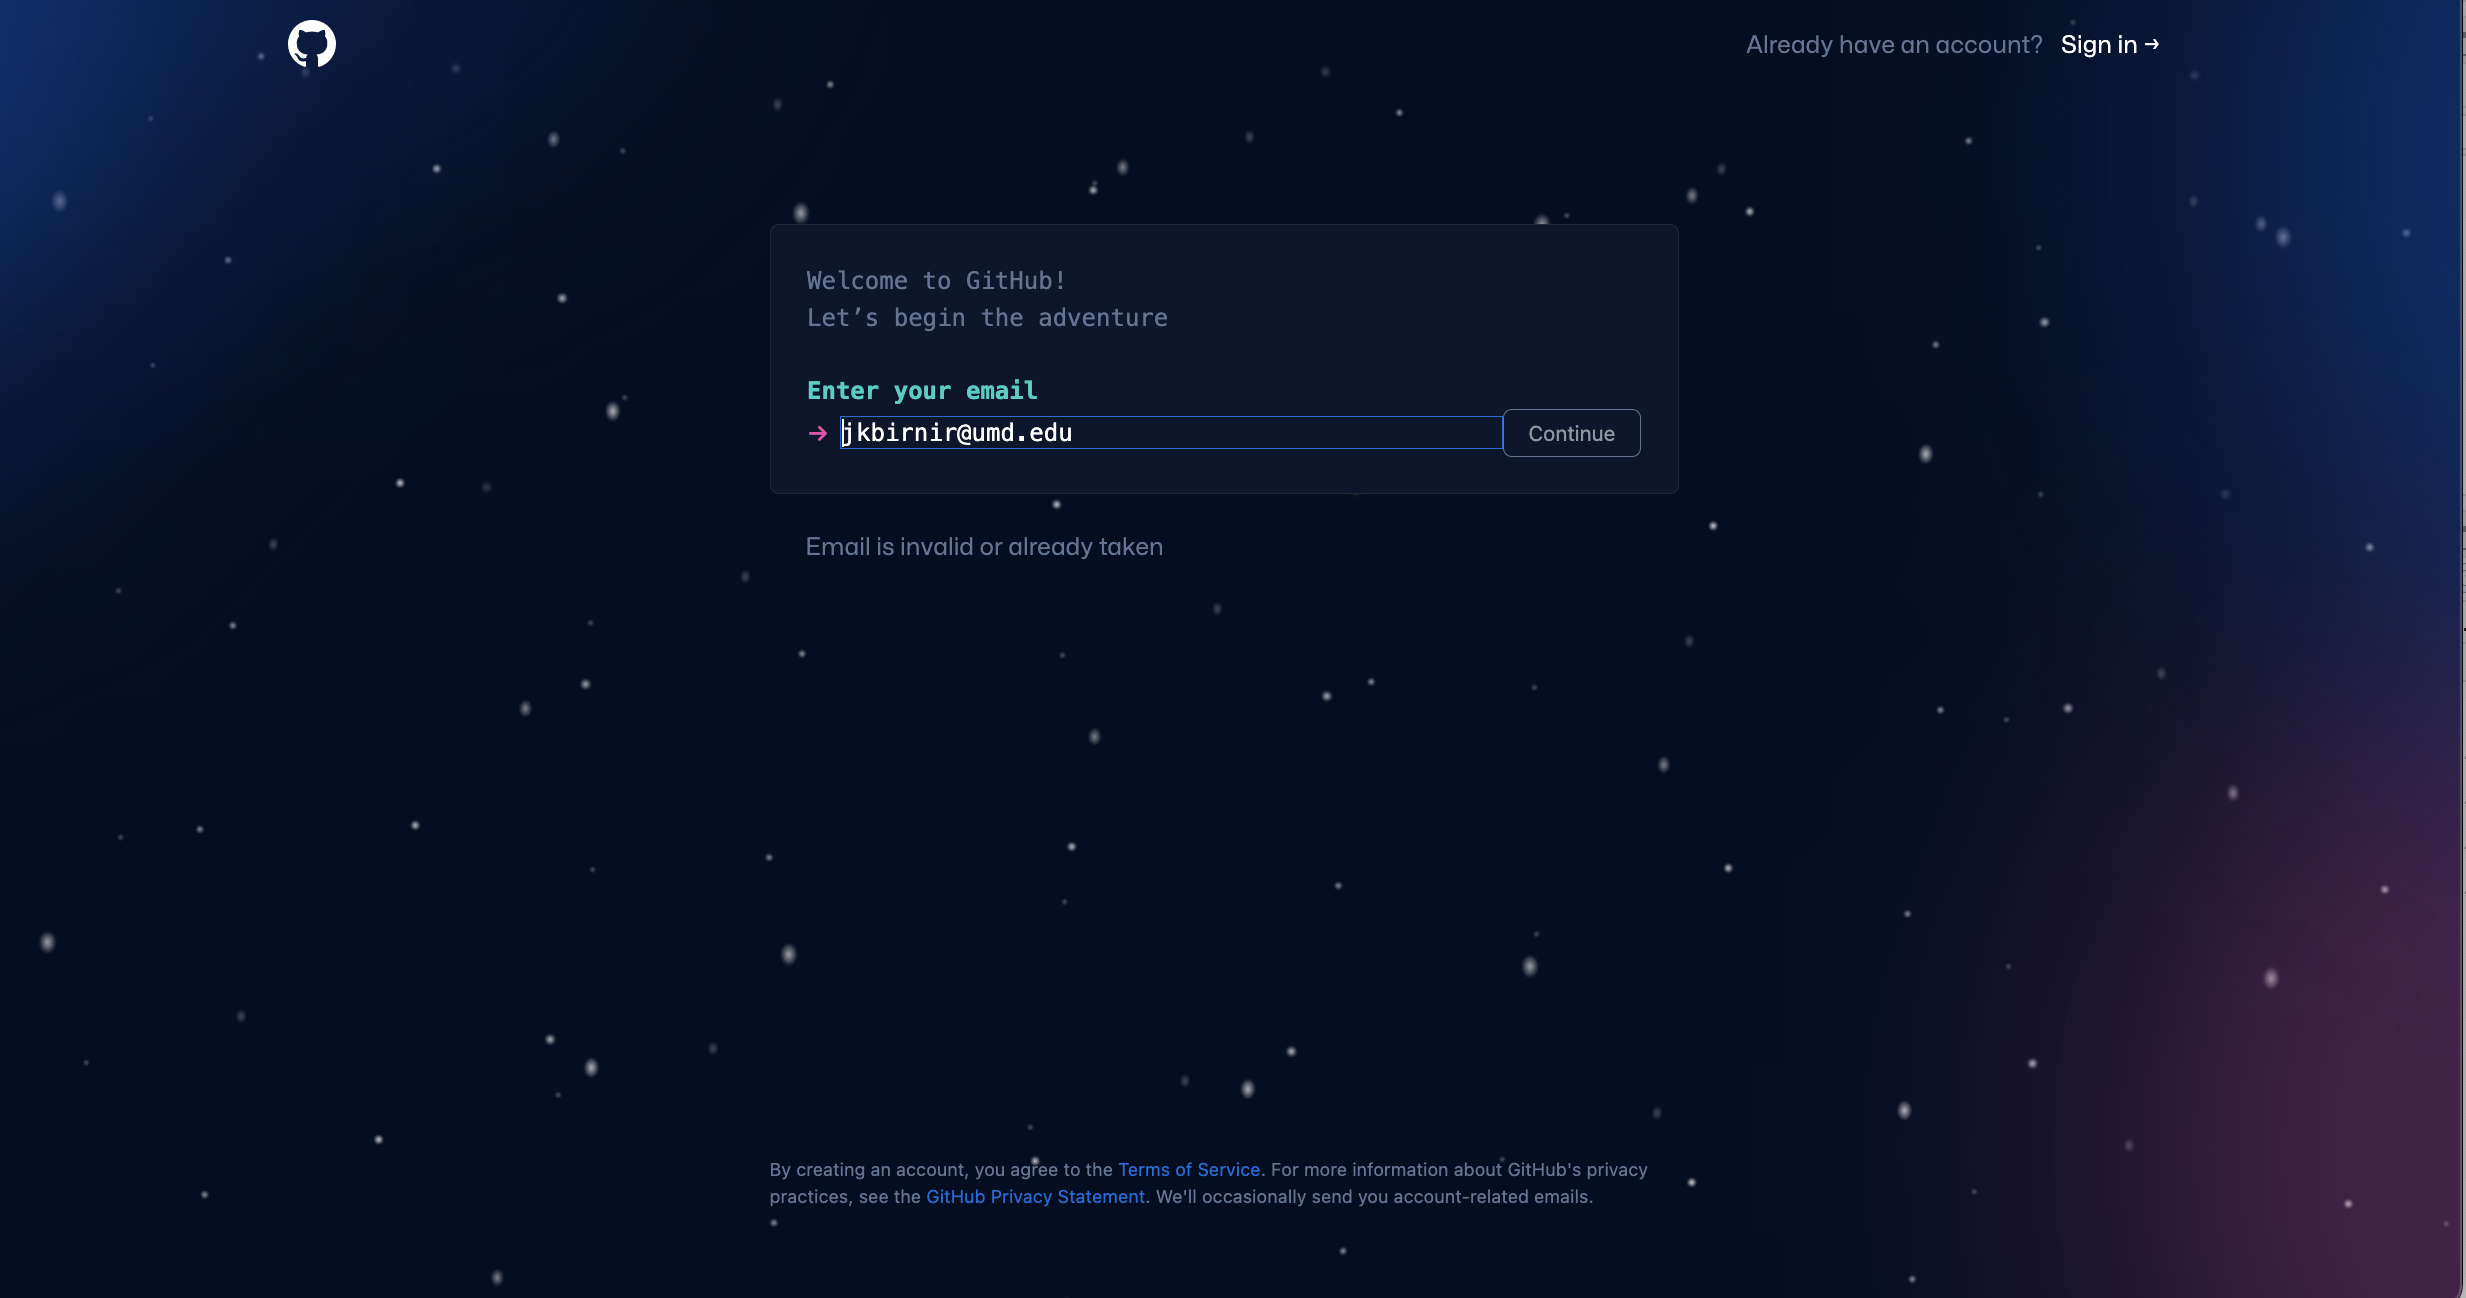
\includegraphics{figures/2.PNG}

}

\caption{Github signup}

\end{figure}

Once you have a github site, in the upper left hand corner on your
github site create a repository for where you want files from your
pending project to go. Name the repository whatever you will be calling
your project. Select to have a readme file where you can post notes
about the project. Select to make it private while you are working on
int (this can be changed later).

\begin{figure}

{\centering 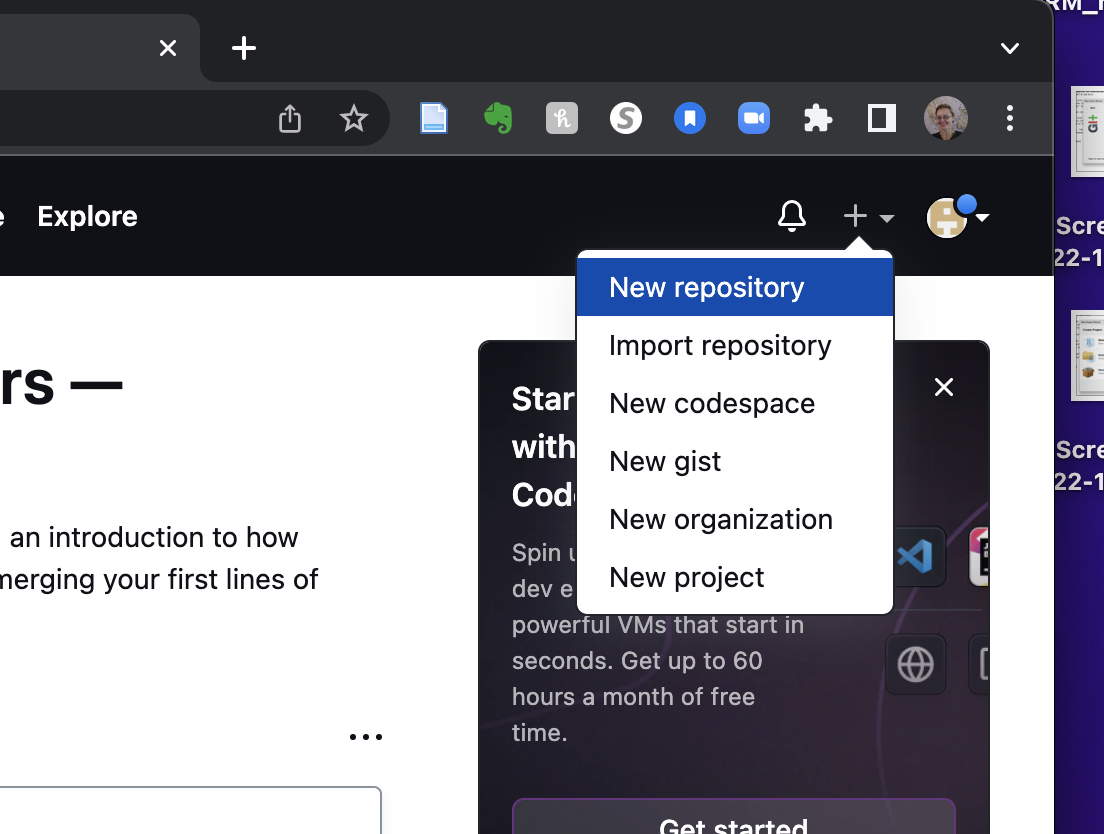
\includegraphics{figures/3.PNG}

}

\caption{Github new repository}

\end{figure}

Once you hit create you new repository should look something like this:

\begin{figure}

{\centering 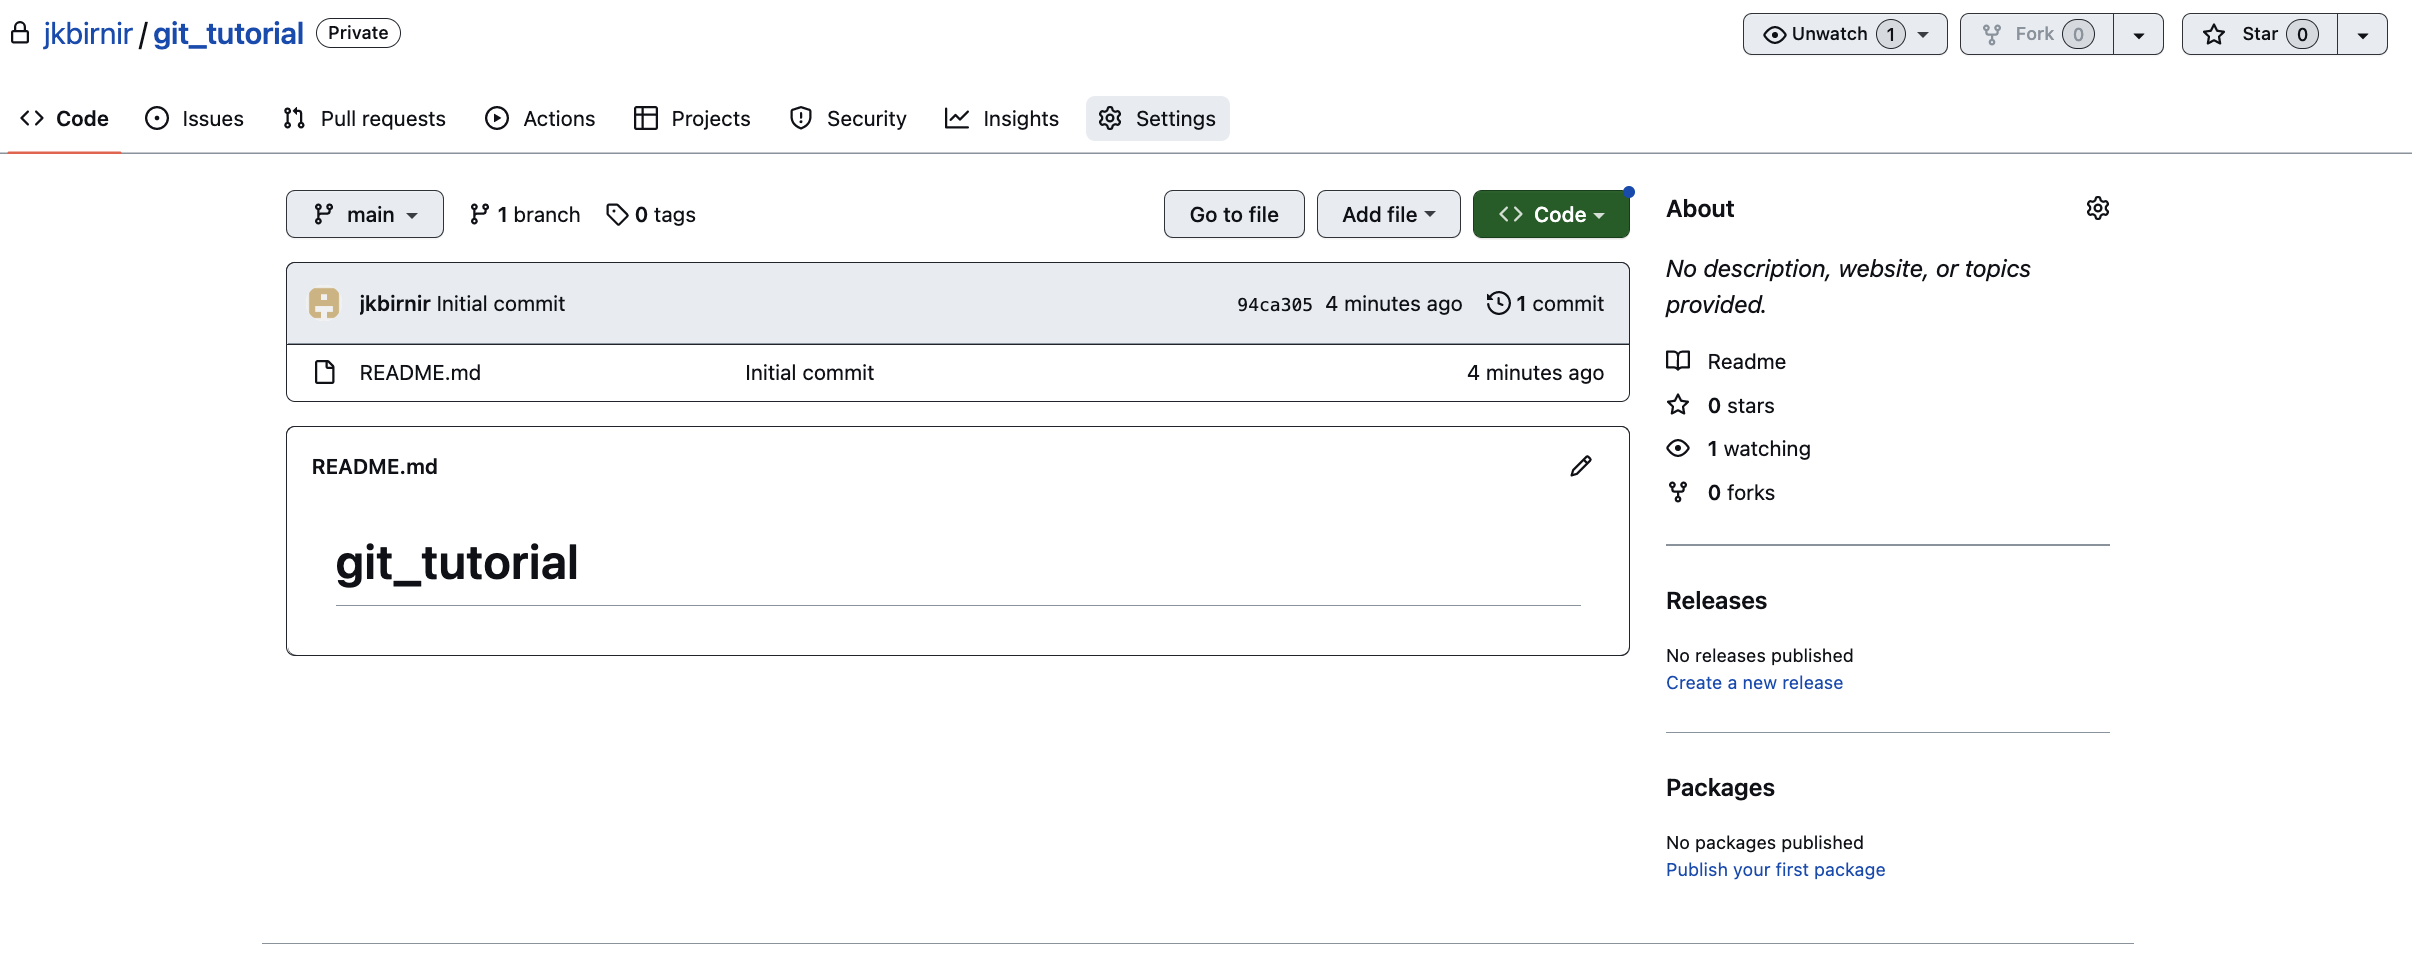
\includegraphics{figures/4.PNG}

}

\caption{terminal git version}

\end{figure}

\hypertarget{getting-started-with-git-on-your-computer}{%
\subsection{Getting started with git on your
computer}\label{getting-started-with-git-on-your-computer}}

Check if you have git installed on your computer. For this you have to
use terminal to check. In your terminal write

git --version

and you should get back your version number.

\begin{figure}

{\centering 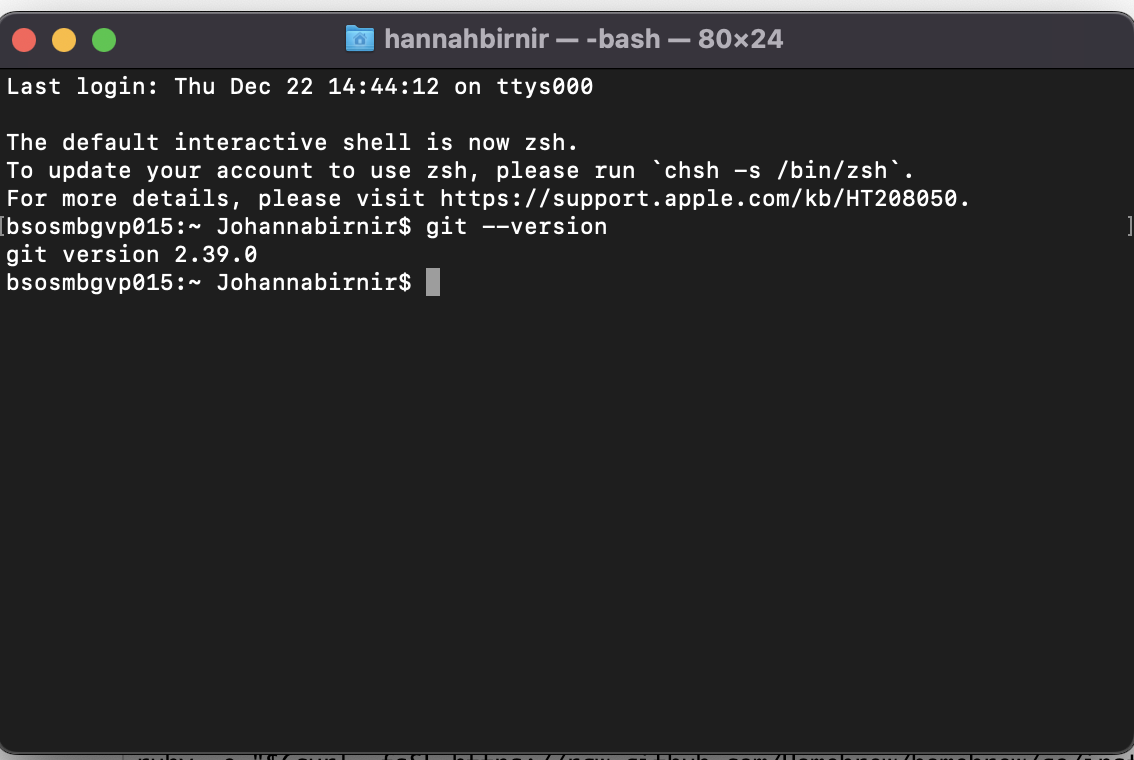
\includegraphics{figures/8.PNG}

}

\caption{terminal git version}

\end{figure}

If you do not have git on your computer you may have to install it. For
instructions on how to check and install git on your computer see this
very helpful
\href{https://jennybc.github.io/2014-05-12-ubc/ubc-r/session03_git.html}{website}
or better yet this \href{https://happygitwithr.com/index.html}{manual}

\hypertarget{setting-up-your-project-in-r-studio}{%
\subsection{Setting up your project in R
studio}\label{setting-up-your-project-in-r-studio}}

Now that you have a github account and a local git on your computer you
are ready to start working with git through R studio.

Open R-studio and start a new project. Choose a project with version
control:

\begin{figure}

{\centering 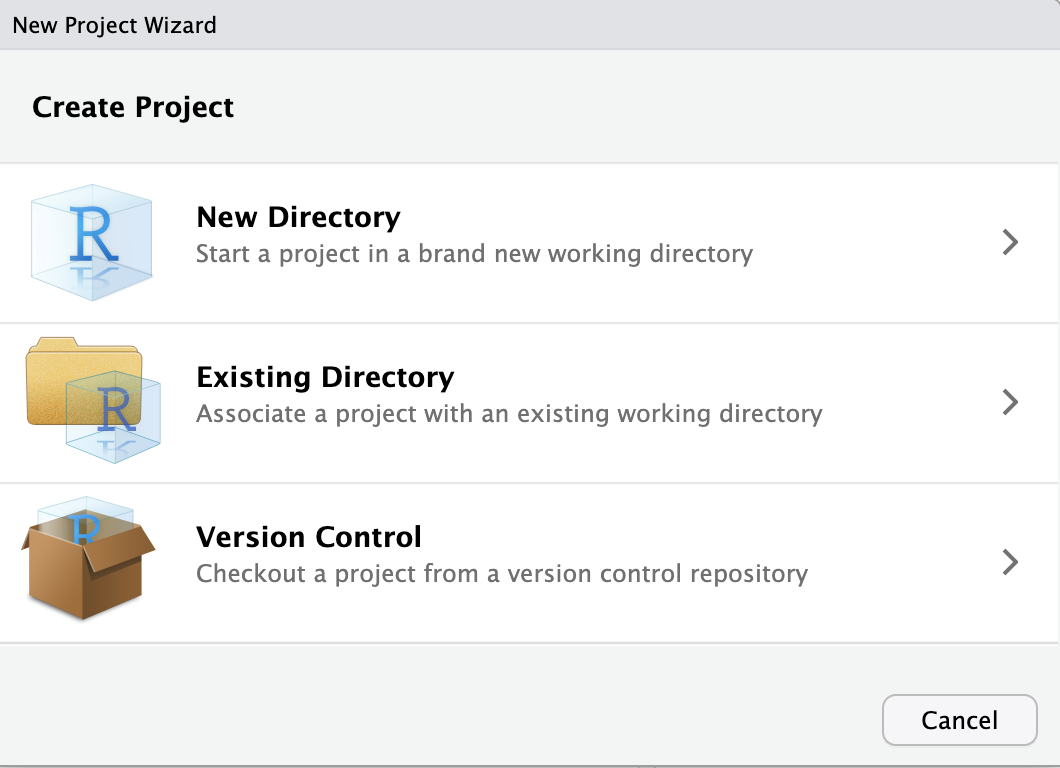
\includegraphics{figures/5.PNG}

}

\caption{Creating a version control project}

\end{figure}

Select the option to clone a repository from git. What R studio will
then do is to clone the repository you created on github locally on your
computer.

\begin{figure}

{\centering 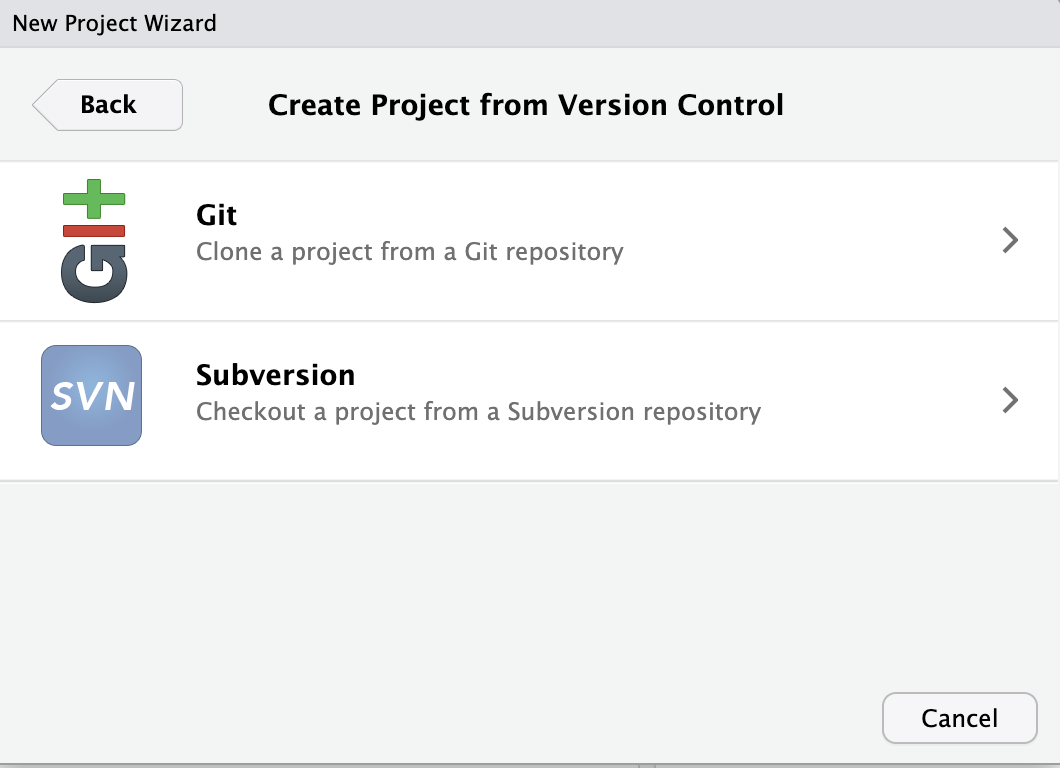
\includegraphics{figures/6.PNG}

}

\caption{Cloning the git repository}

\end{figure}

So that R-studio knows which github local repository to clone you have
to specify an external url that matches your username and the name of
the new repository that you just created on github (Repository URL).

You also have to specify where your local git files are going to be
located see (Create project as subdirectory of:).

\begin{figure}

{\centering 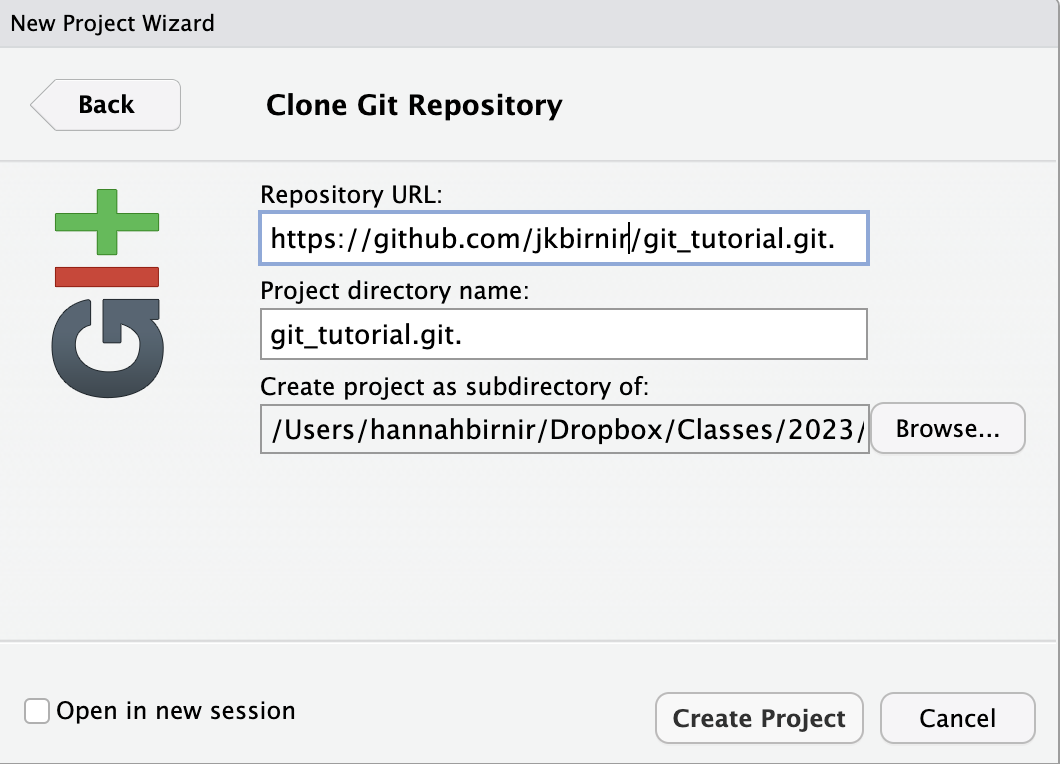
\includegraphics{figures/7.PNG}

}

\caption{Specifying location of external and local repositories}

\end{figure}

Hit the create button and R studio will create a project site that
should look something like this. Notice how the files replicate what is
in

\begin{figure}

{\centering 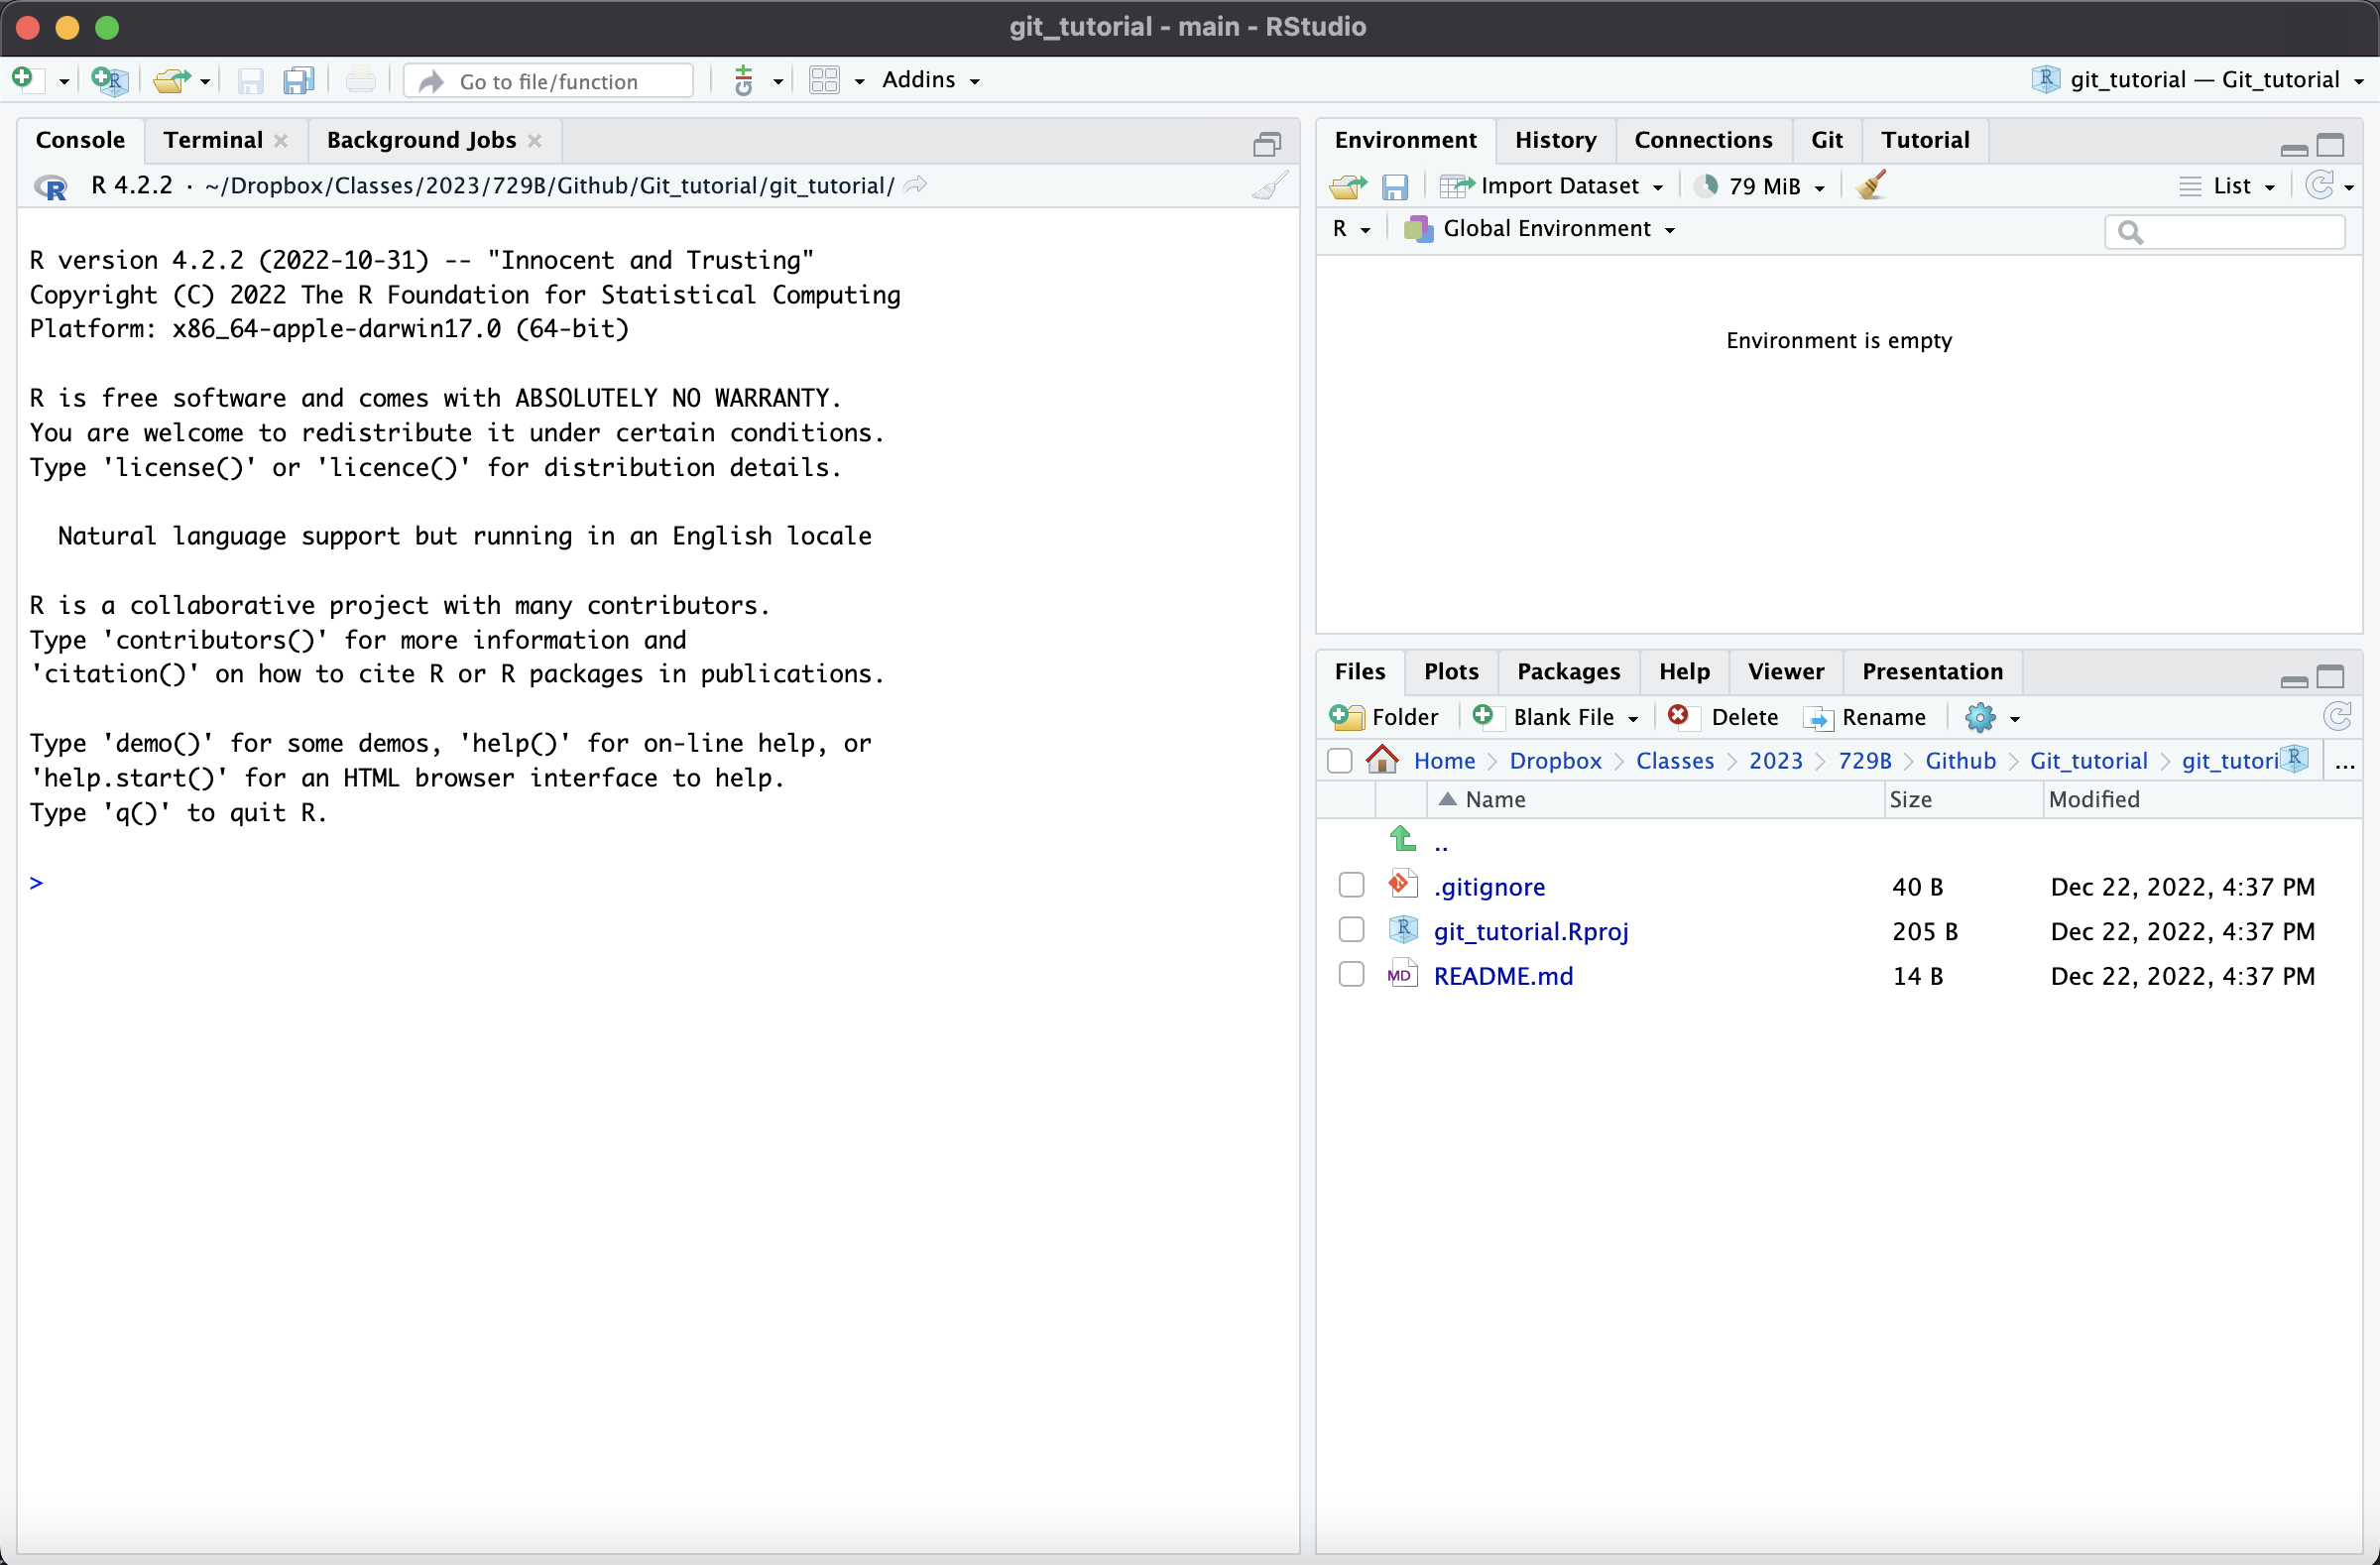
\includegraphics{figures/9.PNG}

}

\caption{local files replicating external repository files}

\end{figure}

In case you run into trouble at this stage - and are not able to connect
your files make sure that your local credentials (signup email matches
the email you used to signup with github). To check this you can use:

\begin{Shaded}
\begin{Highlighting}[]
\FunctionTok{library}\NormalTok{(usethis)}
\FunctionTok{edit\_git\_config}\NormalTok{()}
\end{Highlighting}
\end{Shaded}

\begin{verbatim}
* Edit '/Users/hannahbirnir/.gitconfig'
\end{verbatim}

Remember that you have to install the ``usethis'' package if it is not
already on your computer.

If your git and hub have no problems communicating you can set about
modifying your local files at will, adding files and changing them.

\begin{figure}

{\centering 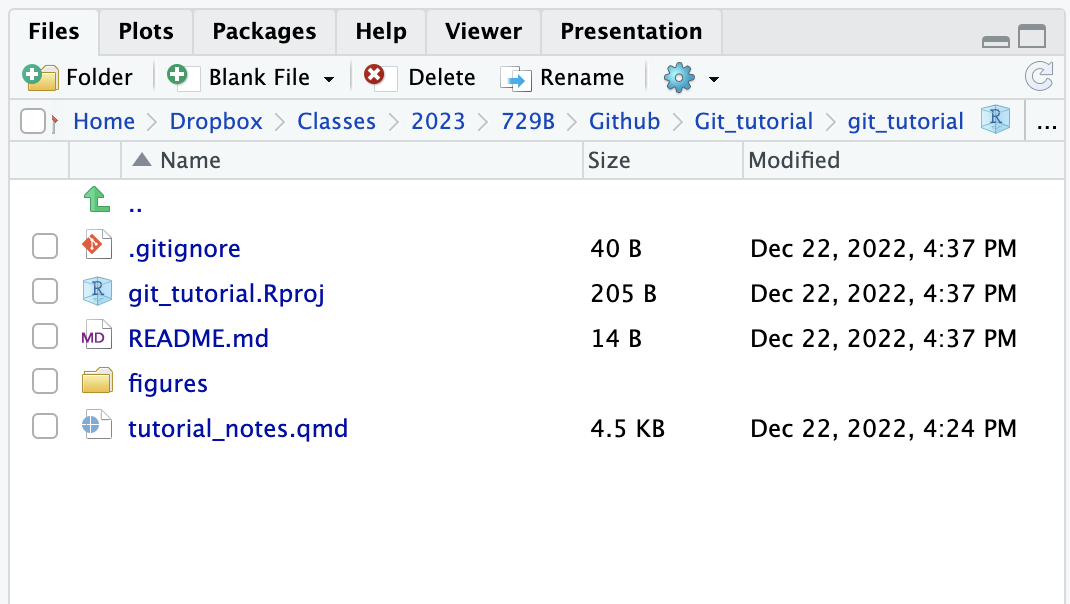
\includegraphics{figures/10.PNG}

}

\caption{Modifying local files}

\end{figure}

Each time you add a new file in your local directory or change it in
some way it will appear in your git tab like so:

\begin{figure}

{\centering 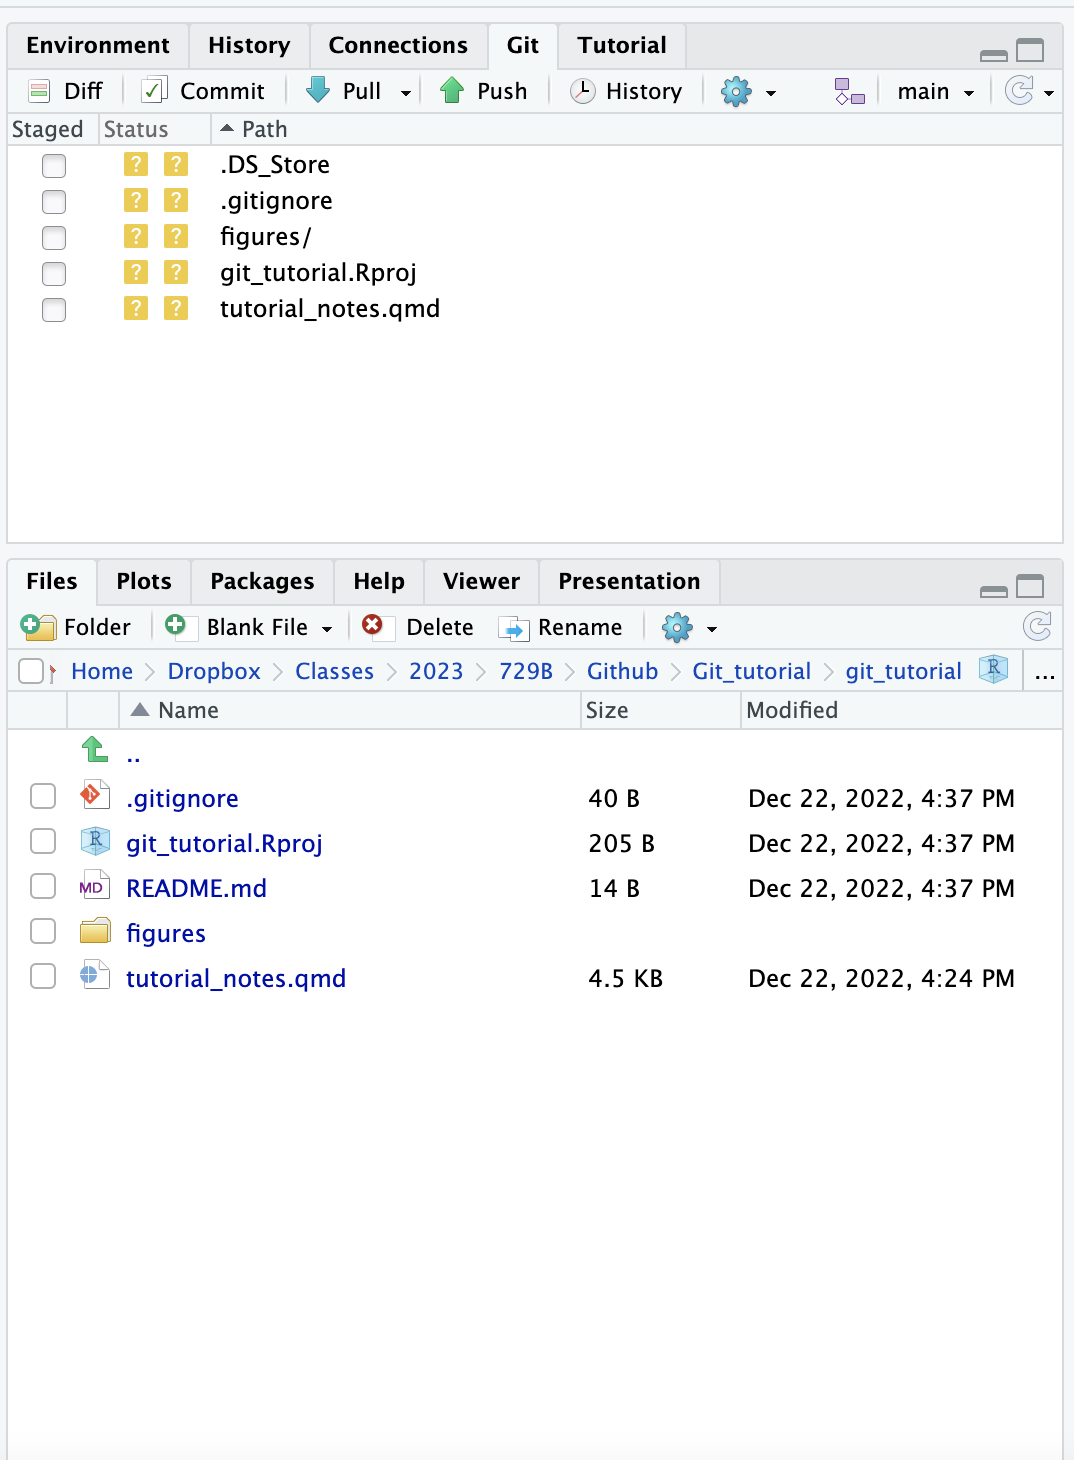
\includegraphics{figures/11.PNG}

}

\caption{Local files in Git tab}

\end{figure}

Notice that because I have not modified the README file that was
imported from github this file does not appear in my git tab.

\hypertarget{pushing-files}{%
\subsection{Pushing files}\label{pushing-files}}

The final step is to commit the changes I have made to my local files to
the github repository. For this purpose I have to commit the files I
want to update (I only commit the files I wish to update) and then I
need to push them to the external repository.

To do this I first select the files that I want to commit. Next I hit
the commit button.

\begin{figure}

{\centering 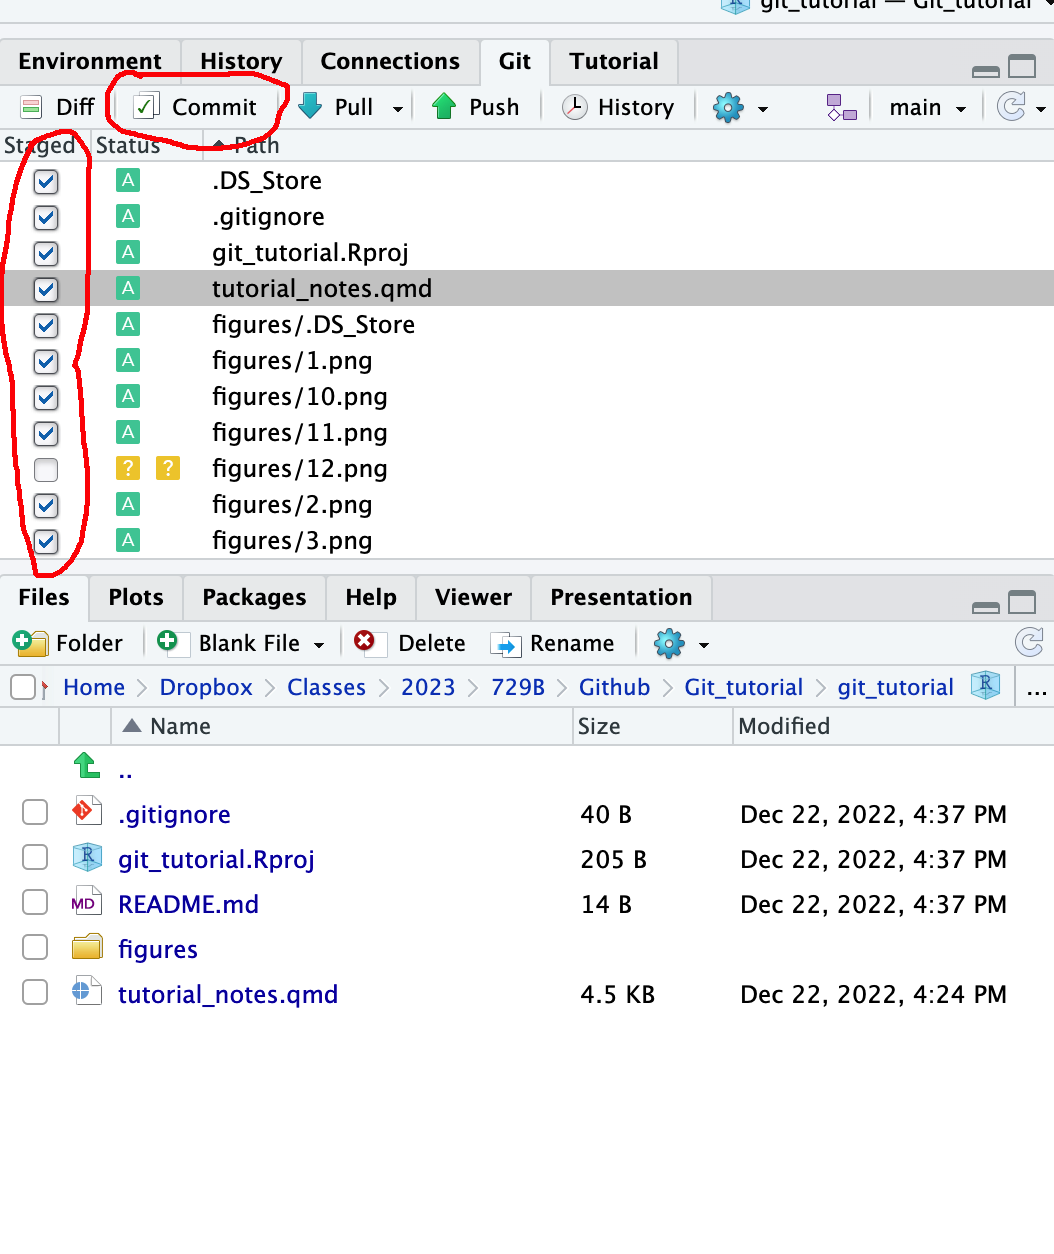
\includegraphics{figures/12.PNG}

}

\caption{Local files in Git tab}

\end{figure}

When I hit the commit button another window pops up where I can write
myself notes about the changes I am committing.

\begin{figure}

{\centering 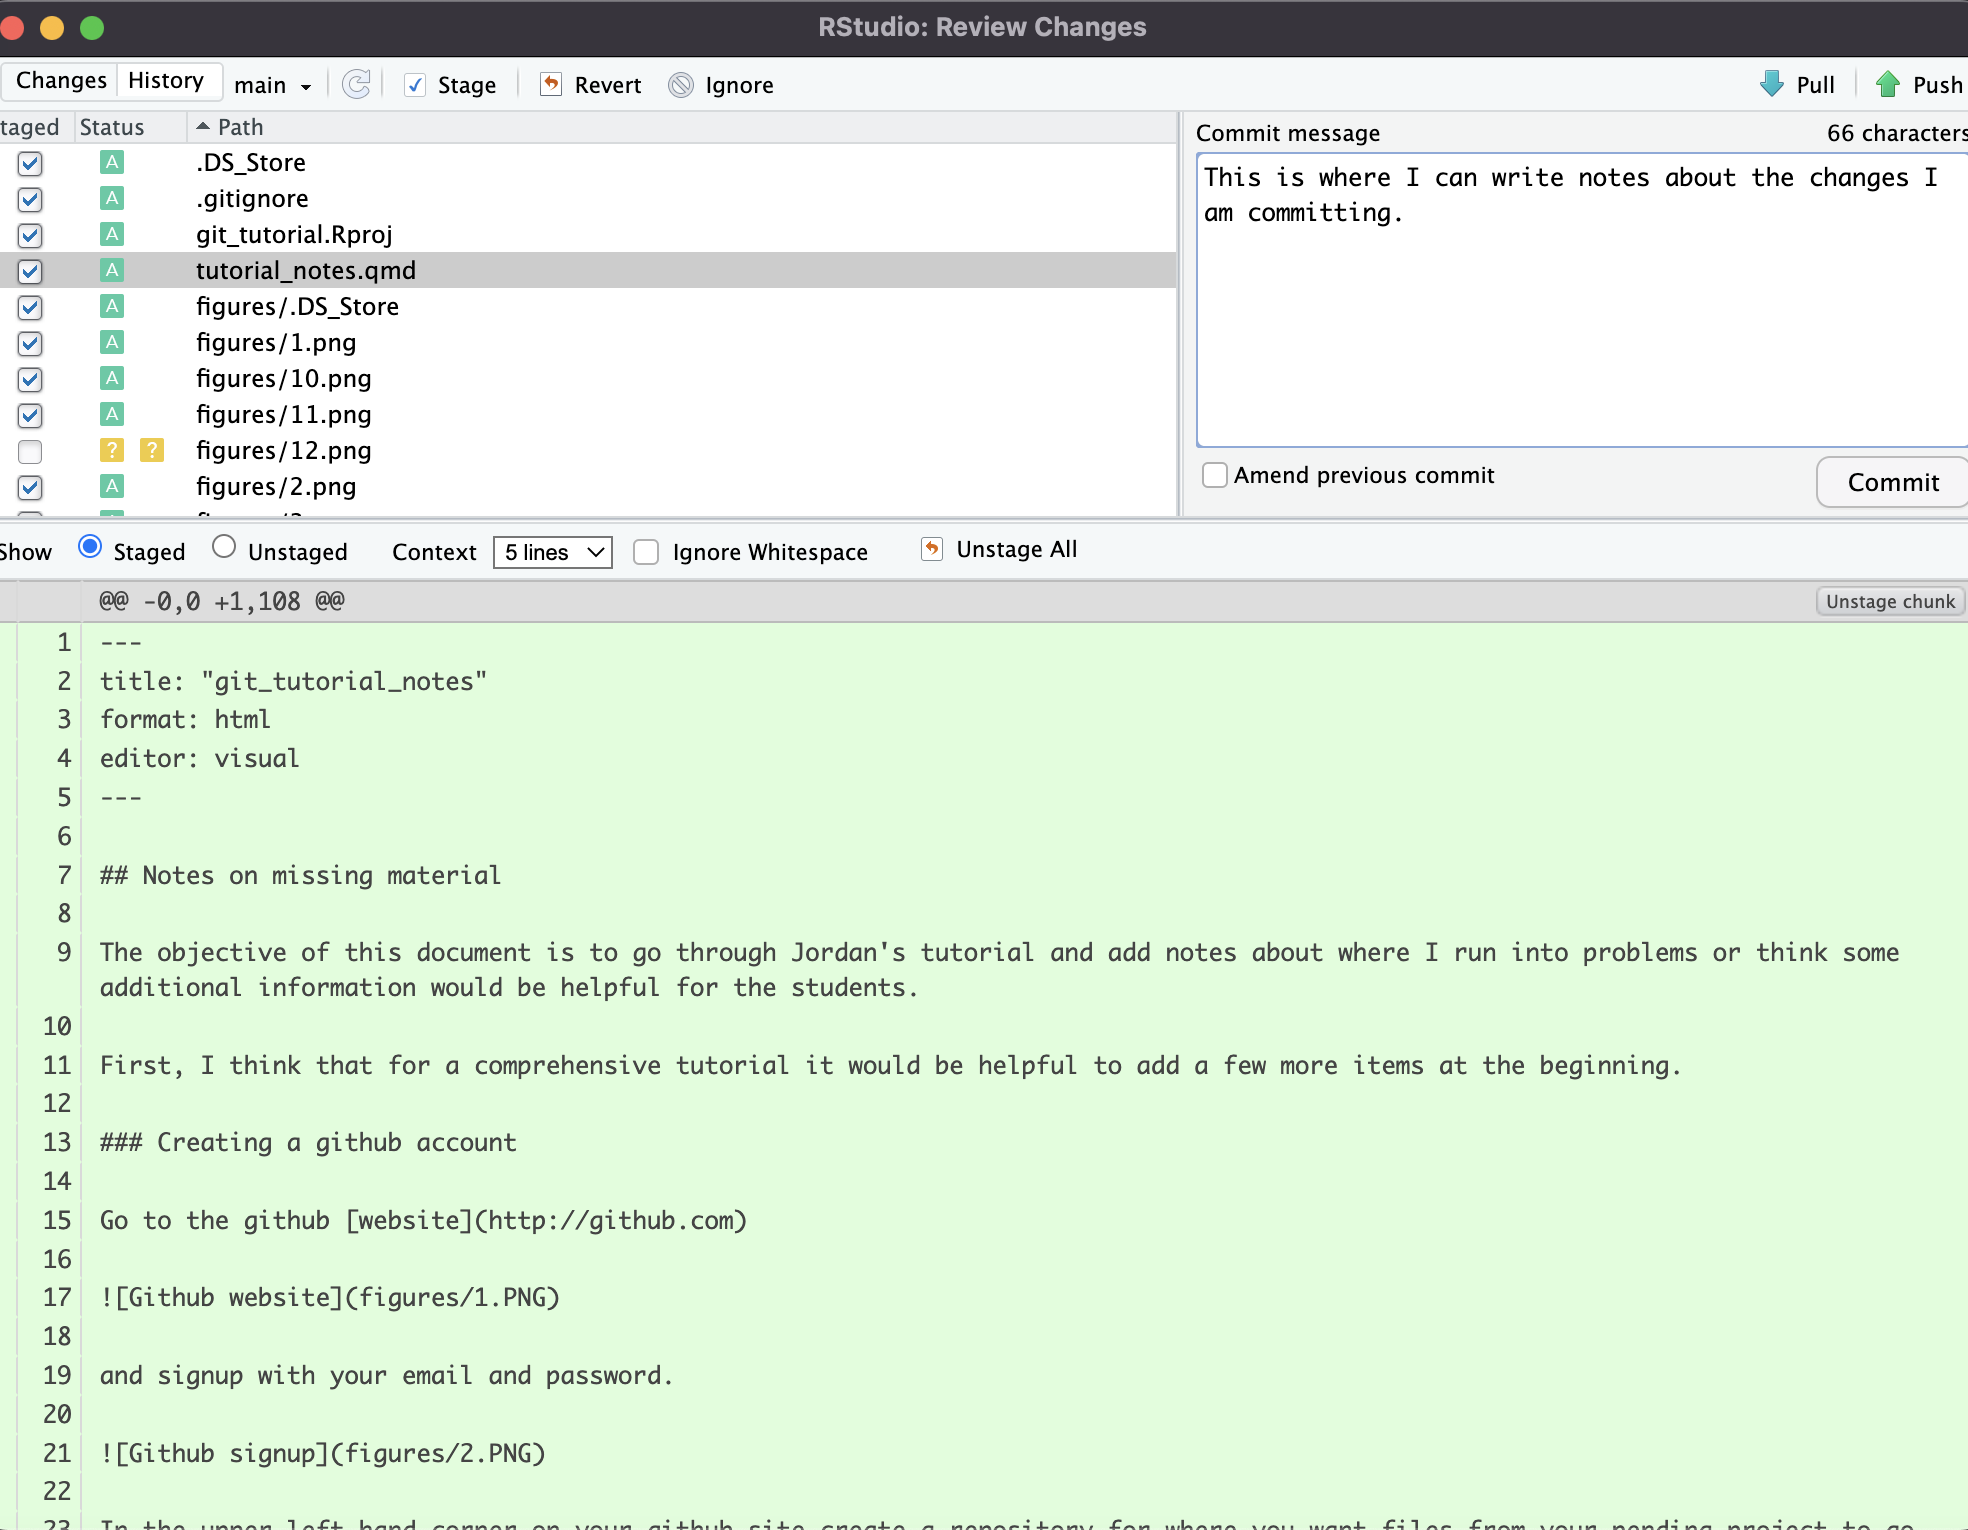
\includegraphics{figures/13.PNG}

}

\caption{Commit notes}

\end{figure}

Once I hit commit R-studio knows which local files I want to change in
my external depository. Note that I can work locally and commit many
files and then work on other files and commit them later. \textbf{Commit
only commits changes to my files locally.} The last step then is to push
all my locally committed files to my external repository.

From within my project I simply push the push button in my now empty git
tab and my external repository is updated.

\begin{figure}

{\centering 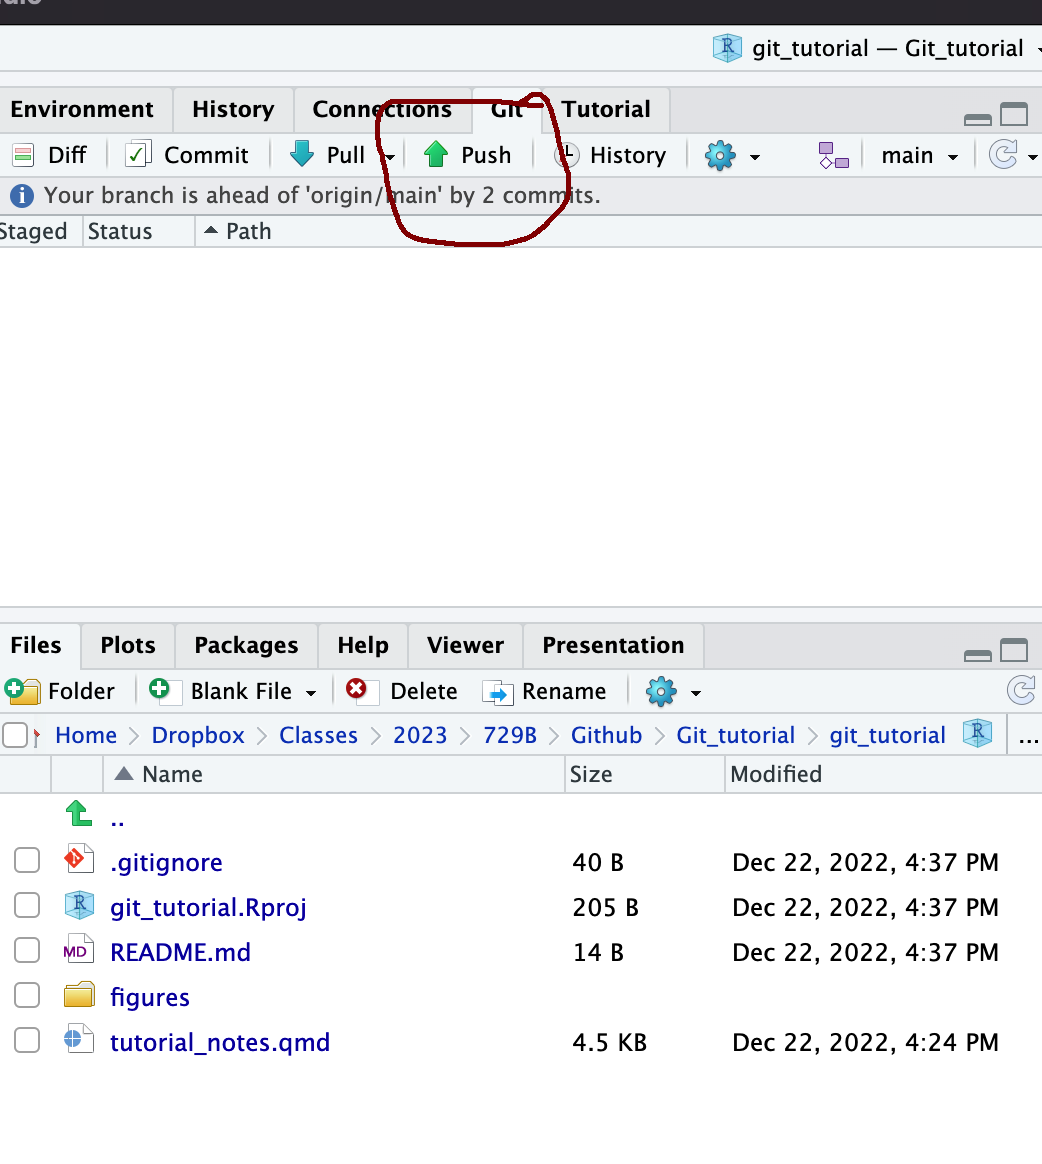
\includegraphics{figures/14.PNG}

}

\caption{Pushing changes to github}

\end{figure}

\begin{figure}

{\centering 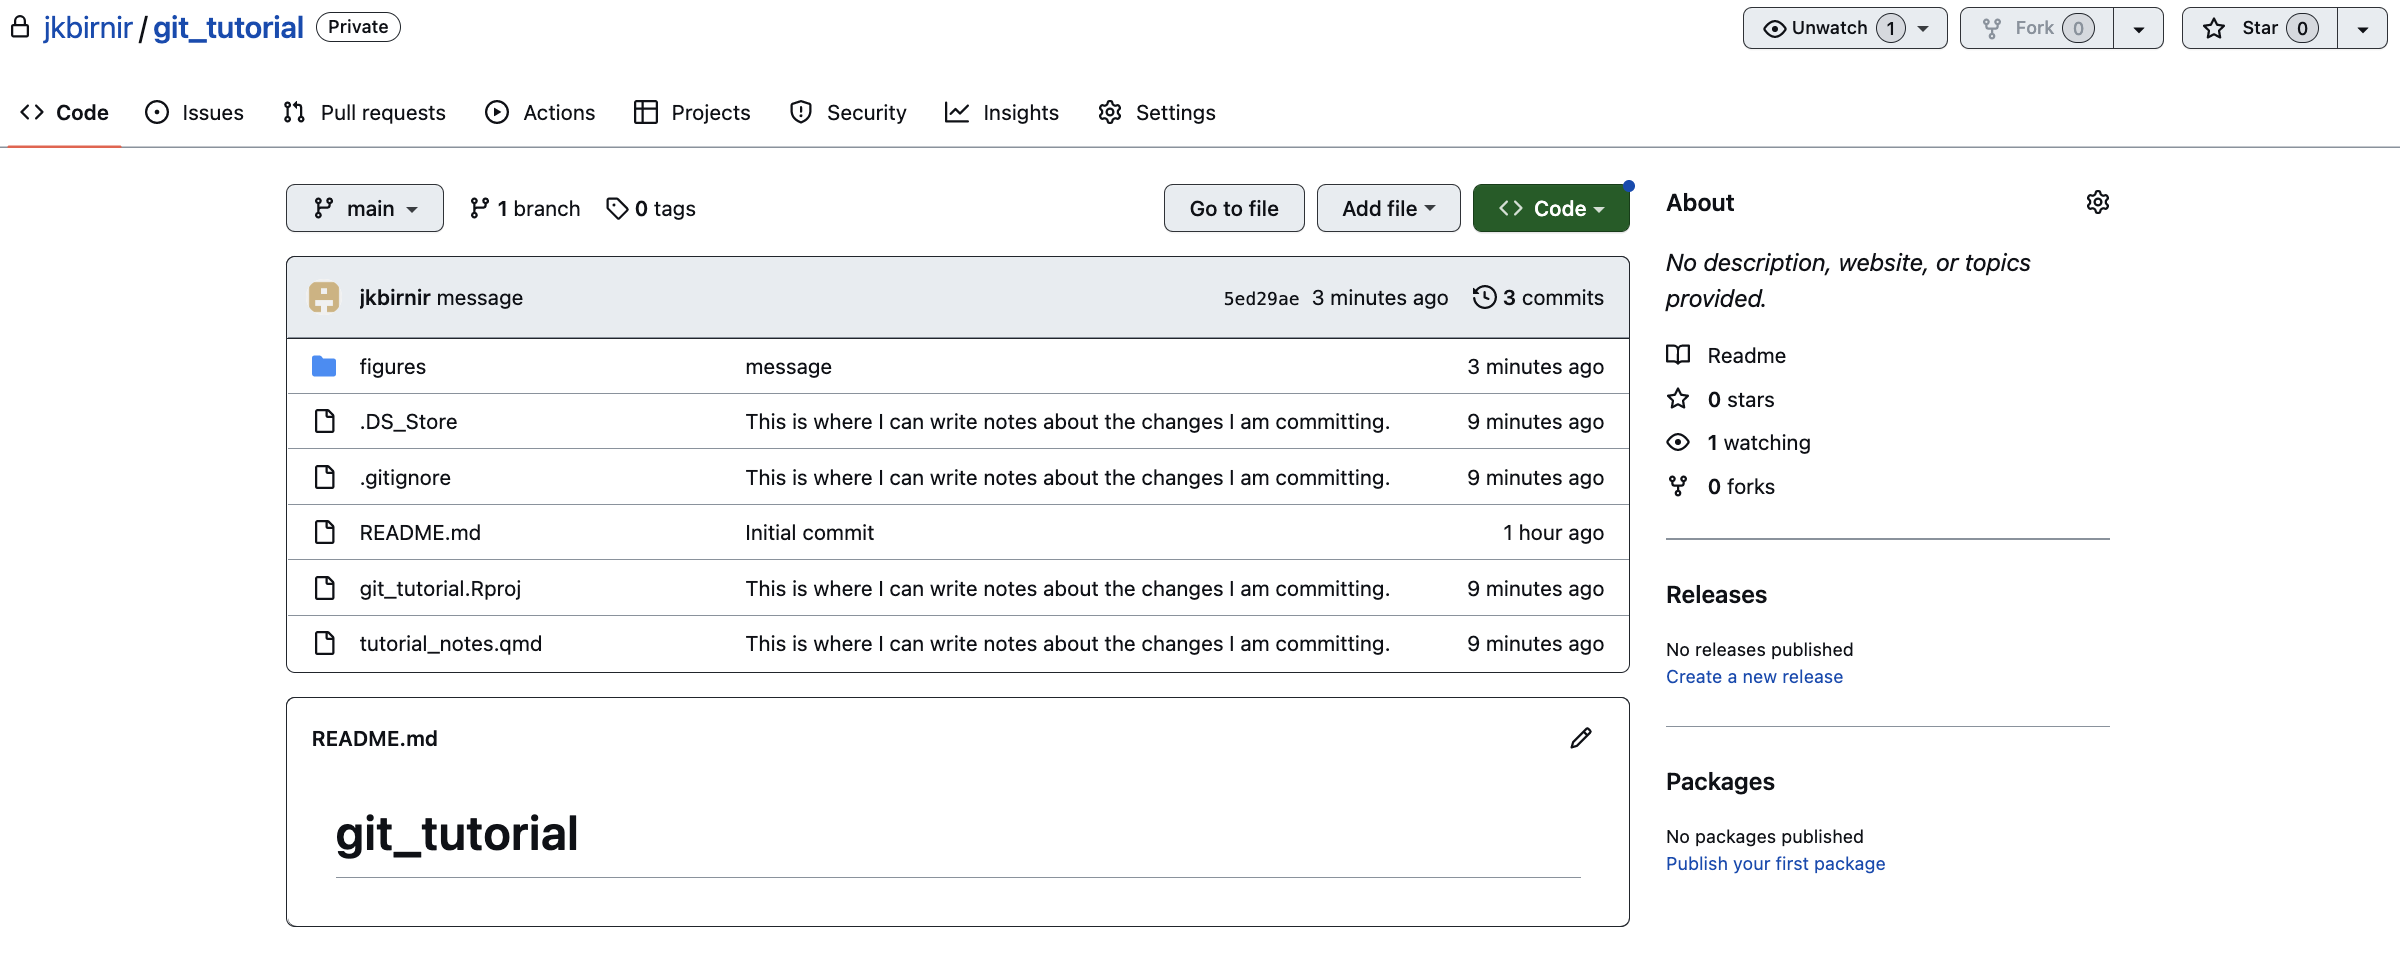
\includegraphics{figures/15.PNG}

}

\caption{Updated external repository}

\end{figure}

Github then tracks all of the changes in each file and new files added
in each commit while also updating the main file.

This is very nice if you are working on a project - like a website that
you might want to change frequently. You can simply open the project -
make a change to any one part of the project and commit those changes to
github. Imagine, for example, a website where you post new data and
other information as it becomes available.

\hypertarget{exercise}{%
\section{Exercise}\label{exercise}}

\hypertarget{install-git-on-your-computer}{%
\subsubsection{Install git on your
computer}\label{install-git-on-your-computer}}

\hypertarget{create-a-github-account}{%
\subsubsection{Create a github account}\label{create-a-github-account}}

\hypertarget{create-a-version-control-project-in-r-studio-and-upload-it-to-github}{%
\subsubsection{Create a version control project in R studio and upload
it to
Github}\label{create-a-version-control-project-in-r-studio-and-upload-it-to-github}}

\hypertarget{working-together-in-git.}{%
\section{Working together in git.}\label{working-together-in-git.}}

One of the most useful things about github is the ability to work
collaboratively.

\hypertarget{associating-your-rstudio-with-a-collaborative-project}{%
\subsection{Associating your RStudio with a collaborative
project}\label{associating-your-rstudio-with-a-collaborative-project}}

First, in order to work collaboratively, you may need to associate your
RStudio with a project in GitHub that you did not create. If you created
the project, do the following to add collaborators:

Go on the Github website to Settings \textgreater{} Manage Access
\textgreater{} Invite a collaborator.

\begin{figure}

{\centering 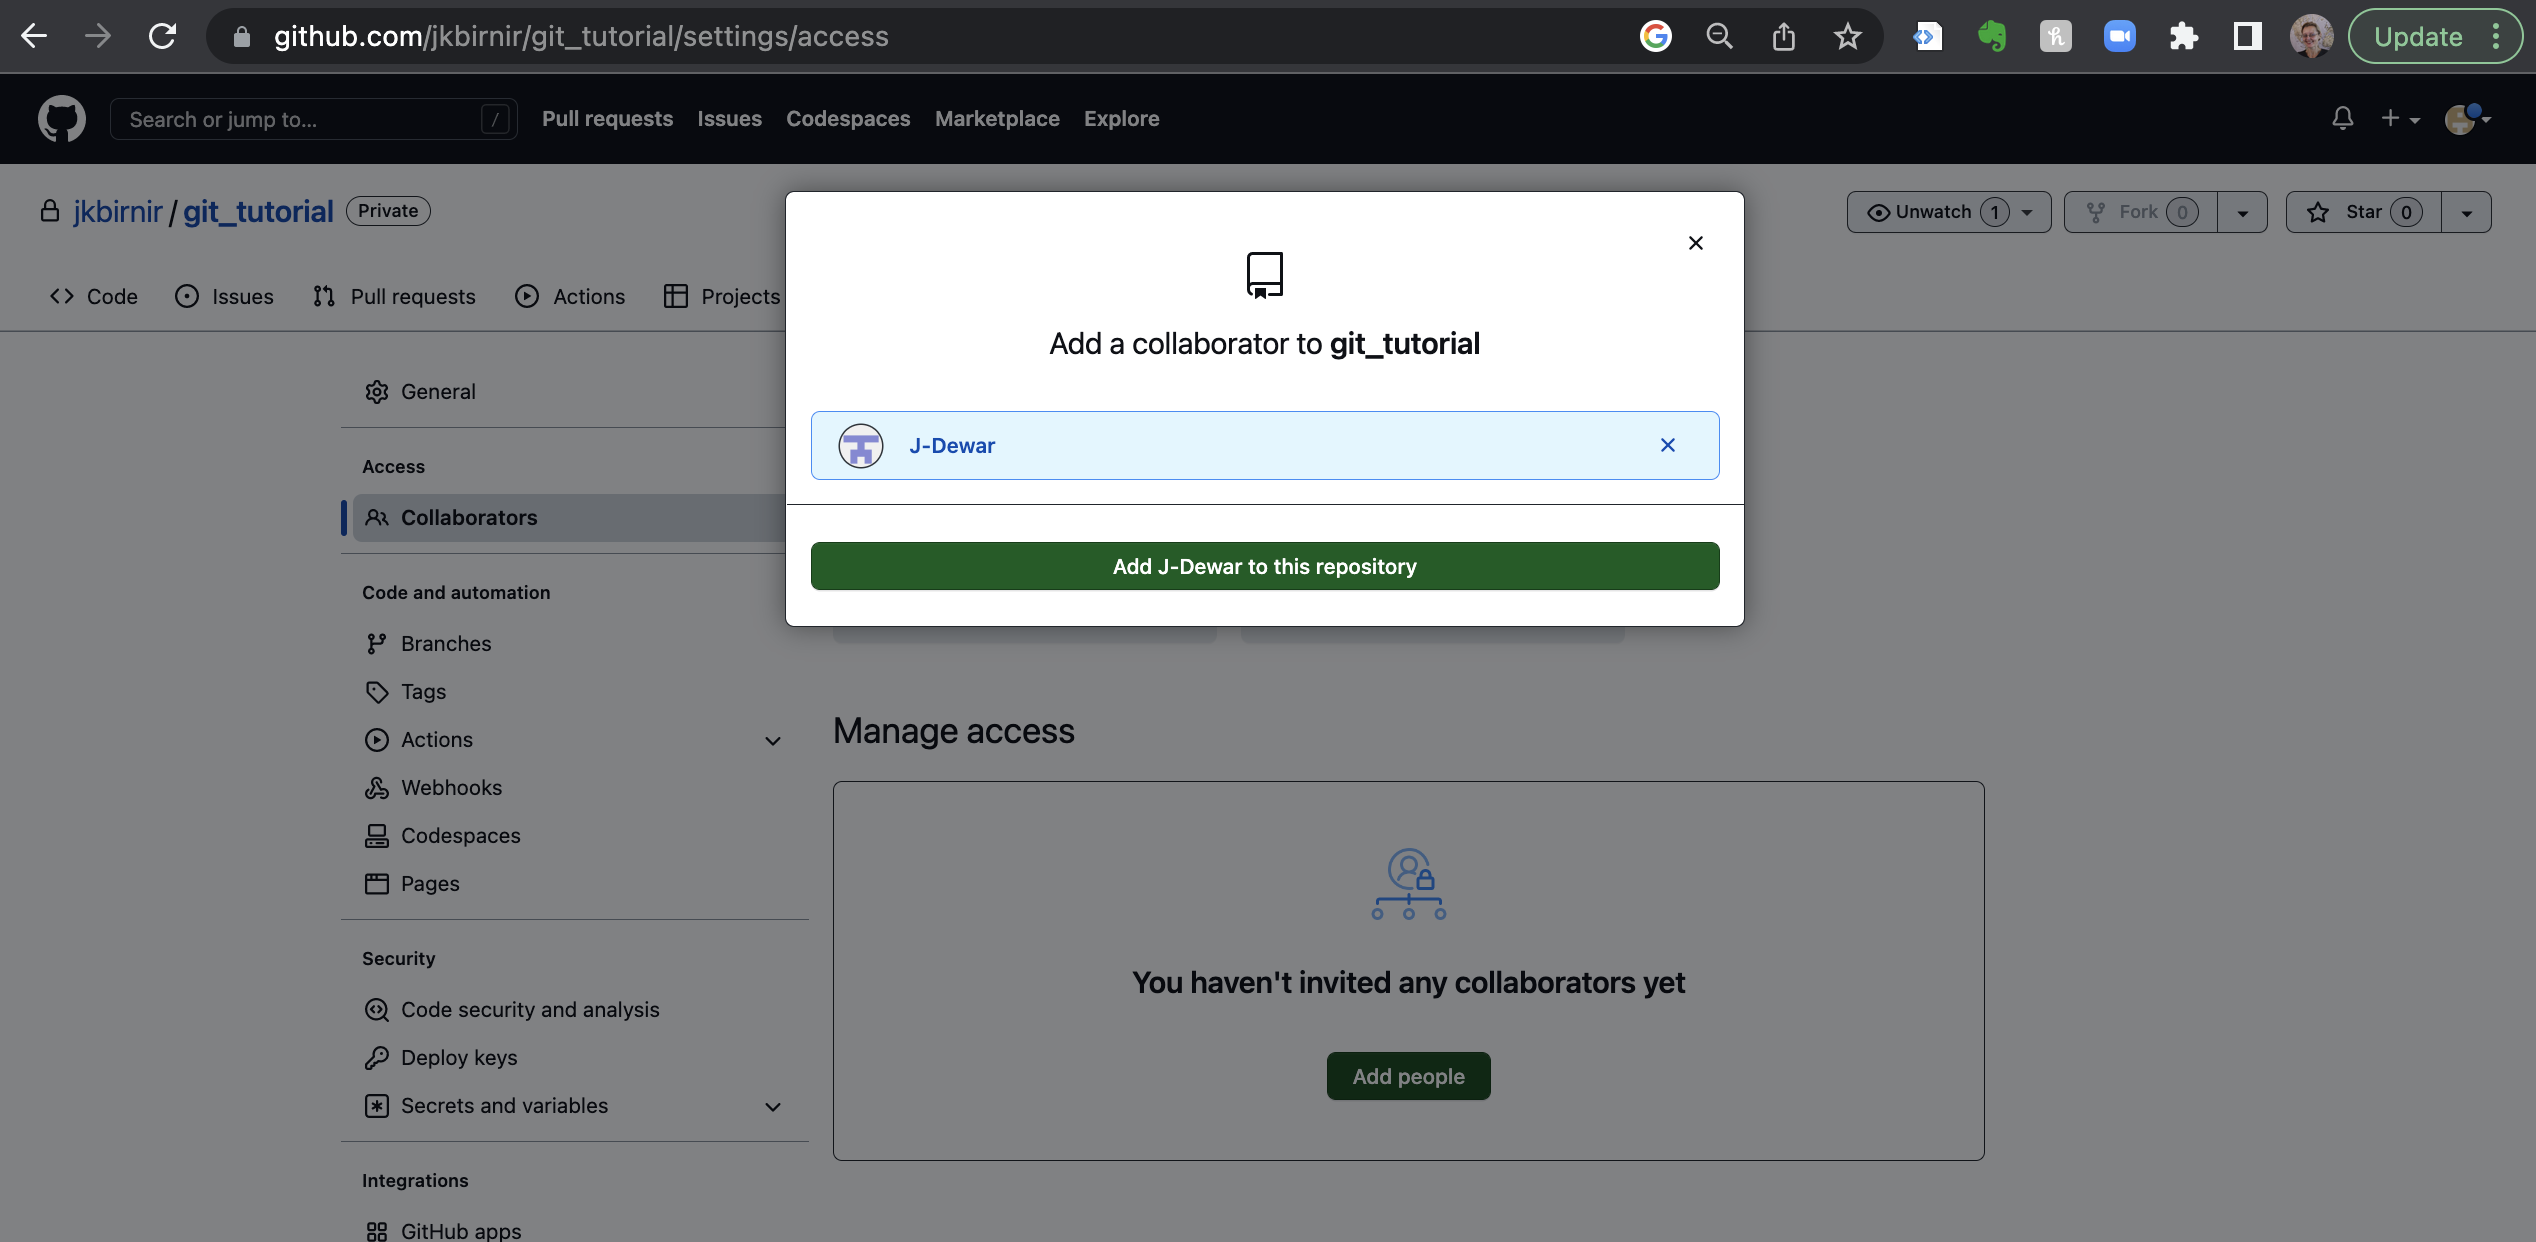
\includegraphics{figures/16.PNG}

}

\caption{Inviting Github Collaborations}

\end{figure}

Your teammate should accept the invite in their email.

Once this is complete, you can use the steps above to associate your
RStuido with the GitHub project.

\hypertarget{pulling-changes}{%
\subsection{Pulling Changes}\label{pulling-changes}}

One important aspect of collaboration in Github is the ability to pull
changes. This allows you to update your code to align with changes
pushed by collaborators.

Using the down arrow button, RStudio goes to the GitHub repo, grabs the
most recent code and brings it into your local editor. (Pulling
regularly is extremely important if you're collaborating, though if
you're the only one working on an RStudio project and associated GitHub
repo, you know your local code matches what's on GitHub so it's less
important.)

To pull, click the blue down arrow on your Git tab to see if you have
changes to pull. If collaborating, you might run into merge conflicts.

When you pull your project updates to show the changes your collaborator
has made to the project. Look at the dates.

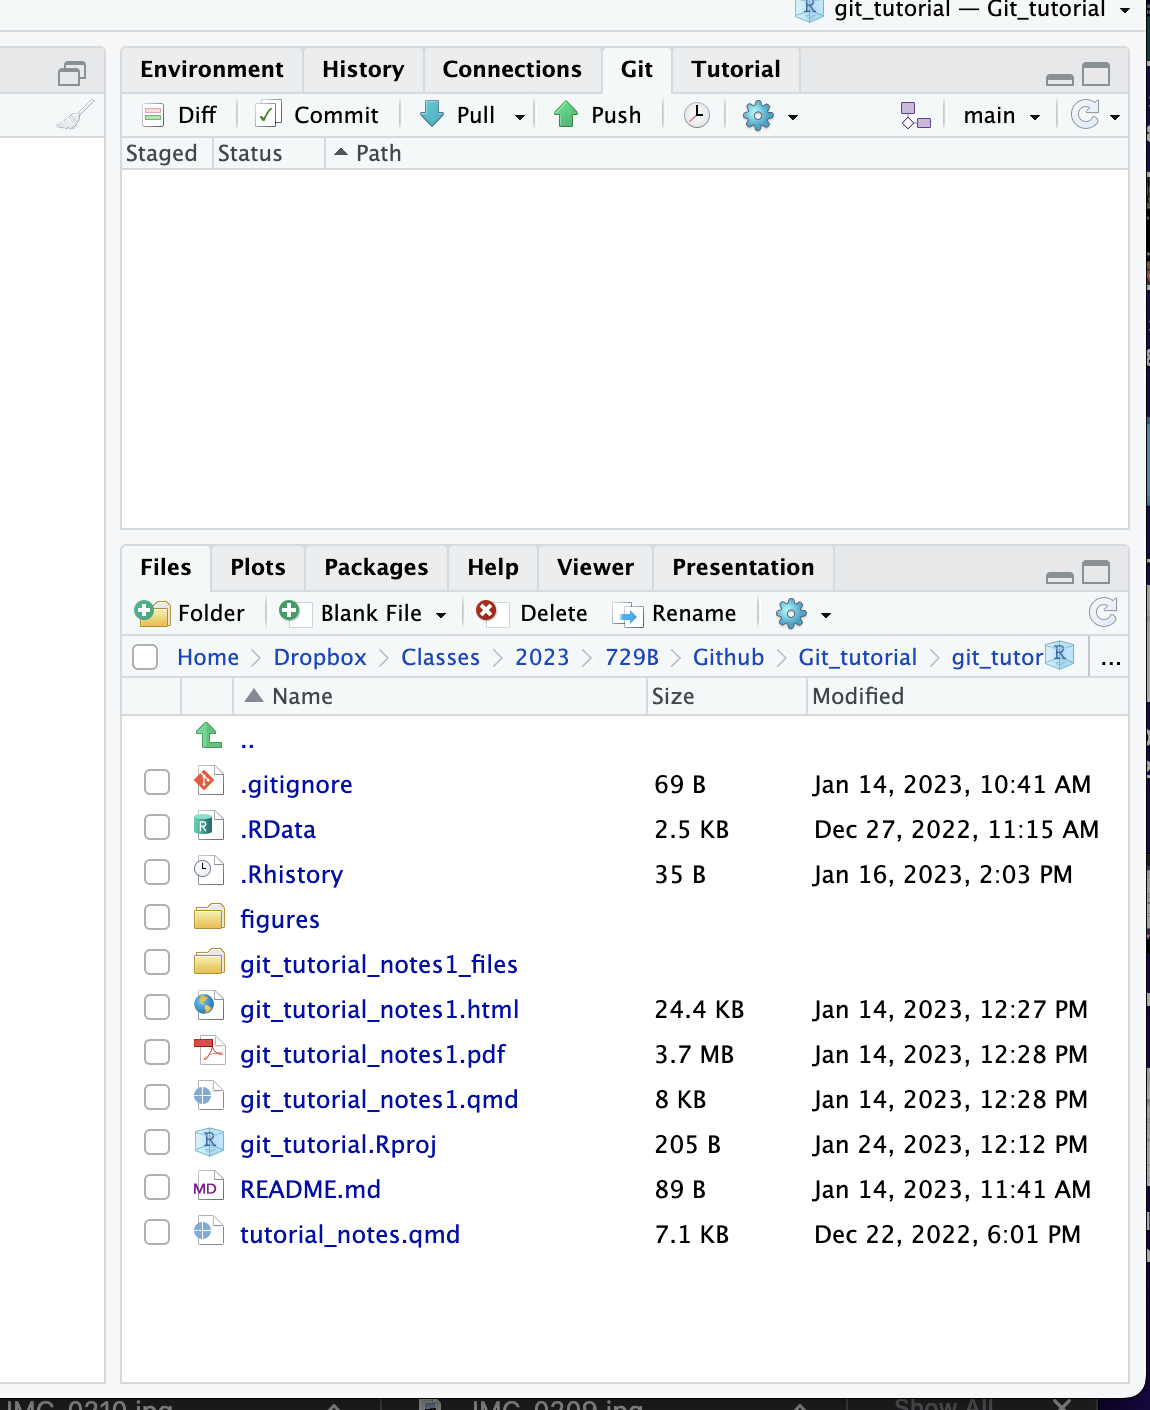
\includegraphics{figures/18.png}

and

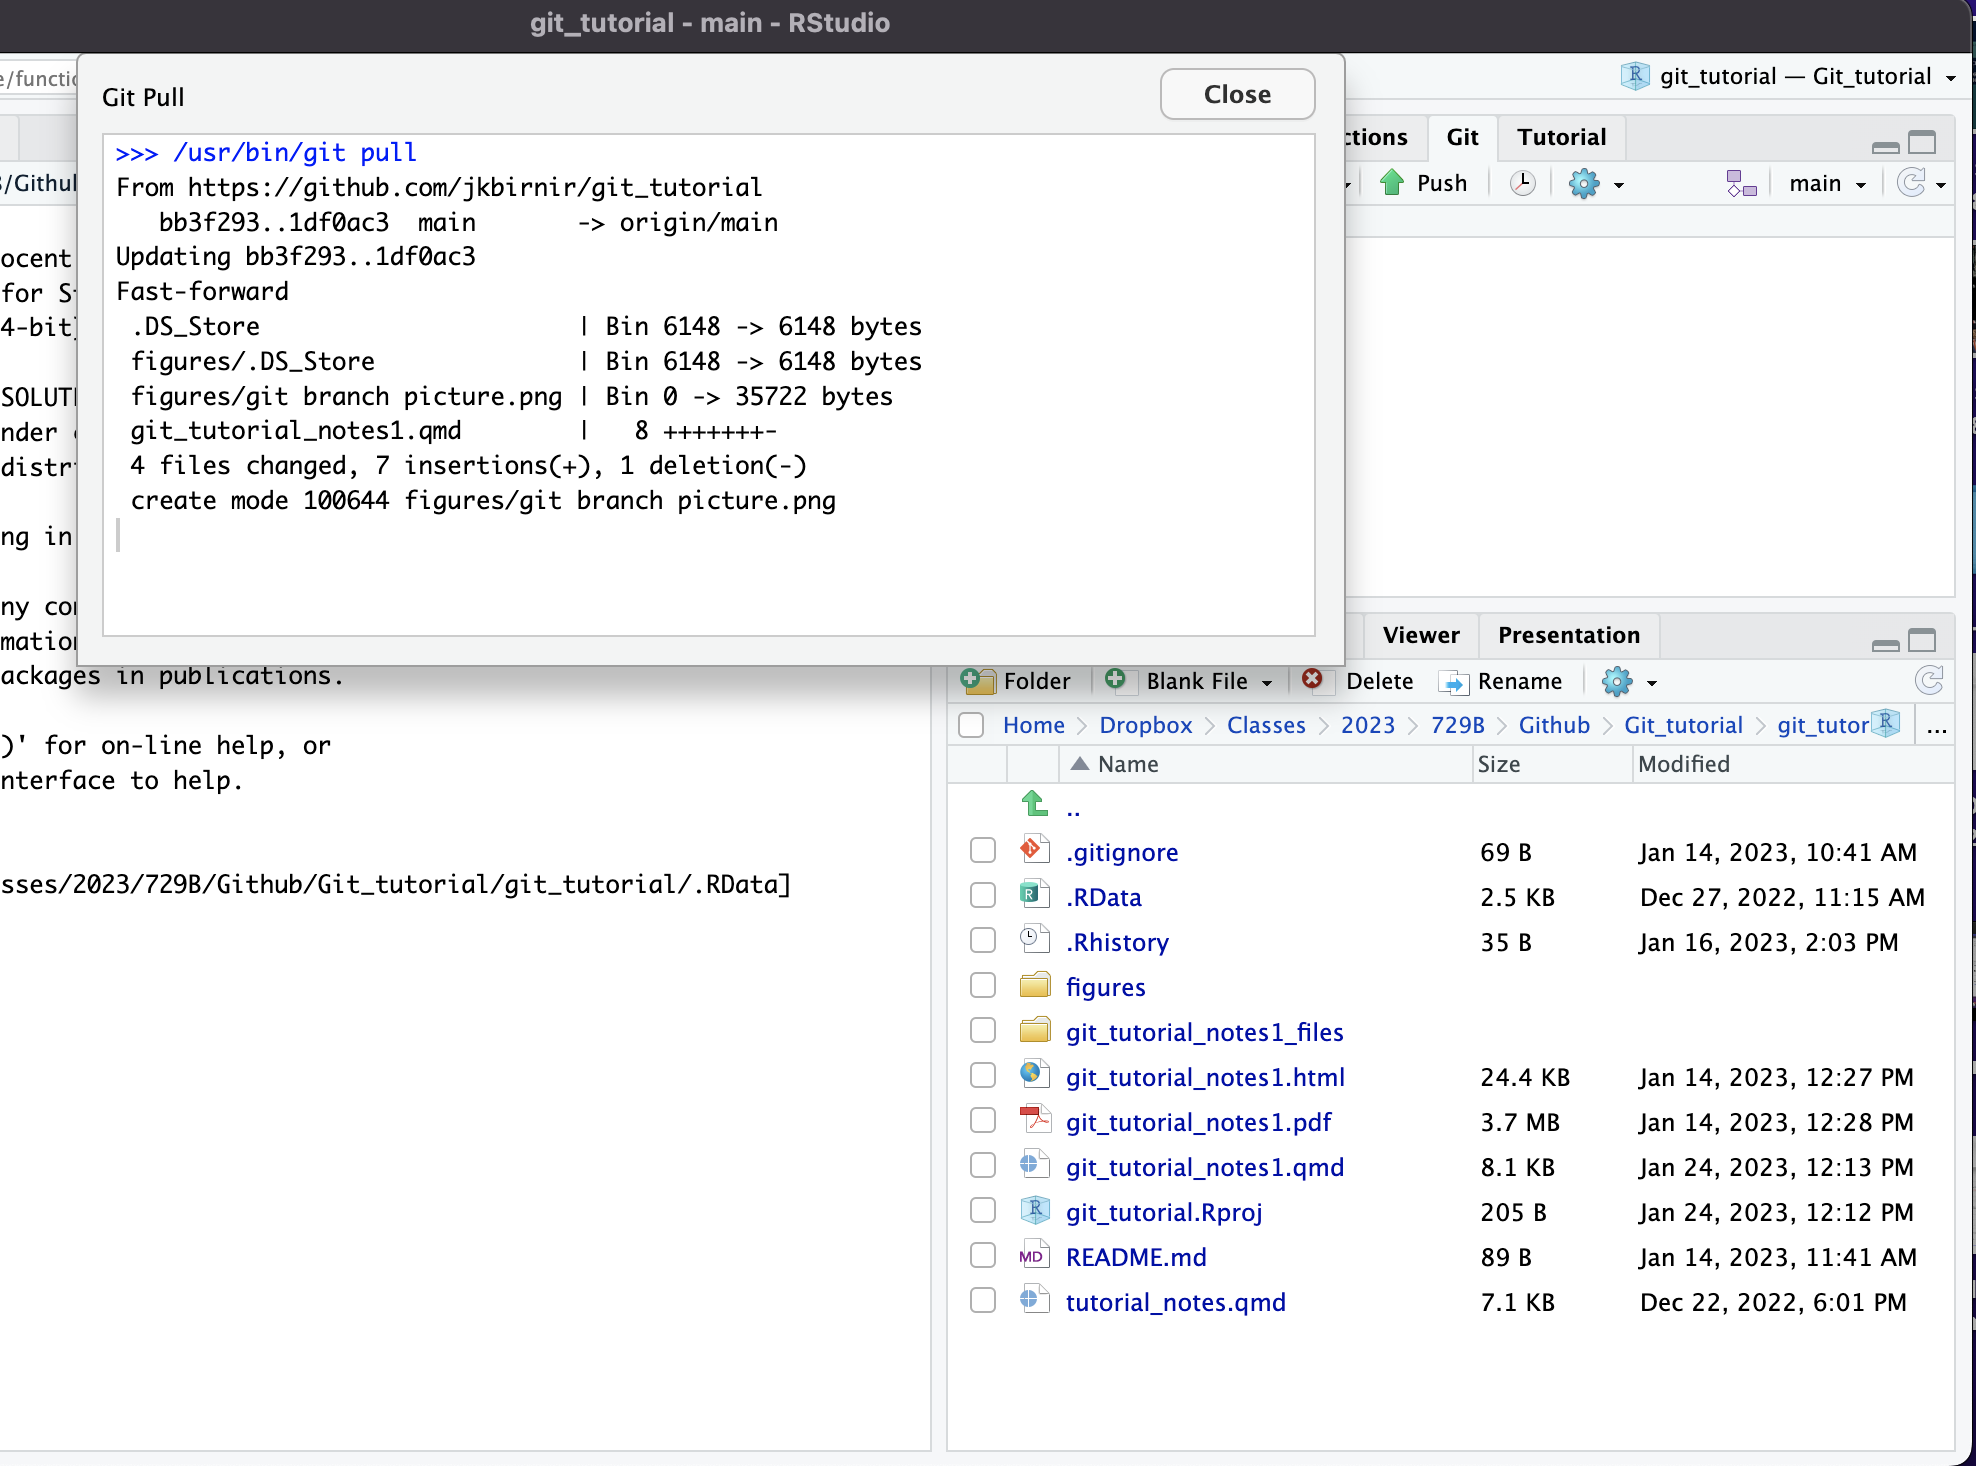
\includegraphics{figures/19.png} You can also track the changes on
github if you want more details.

Go to your github project:

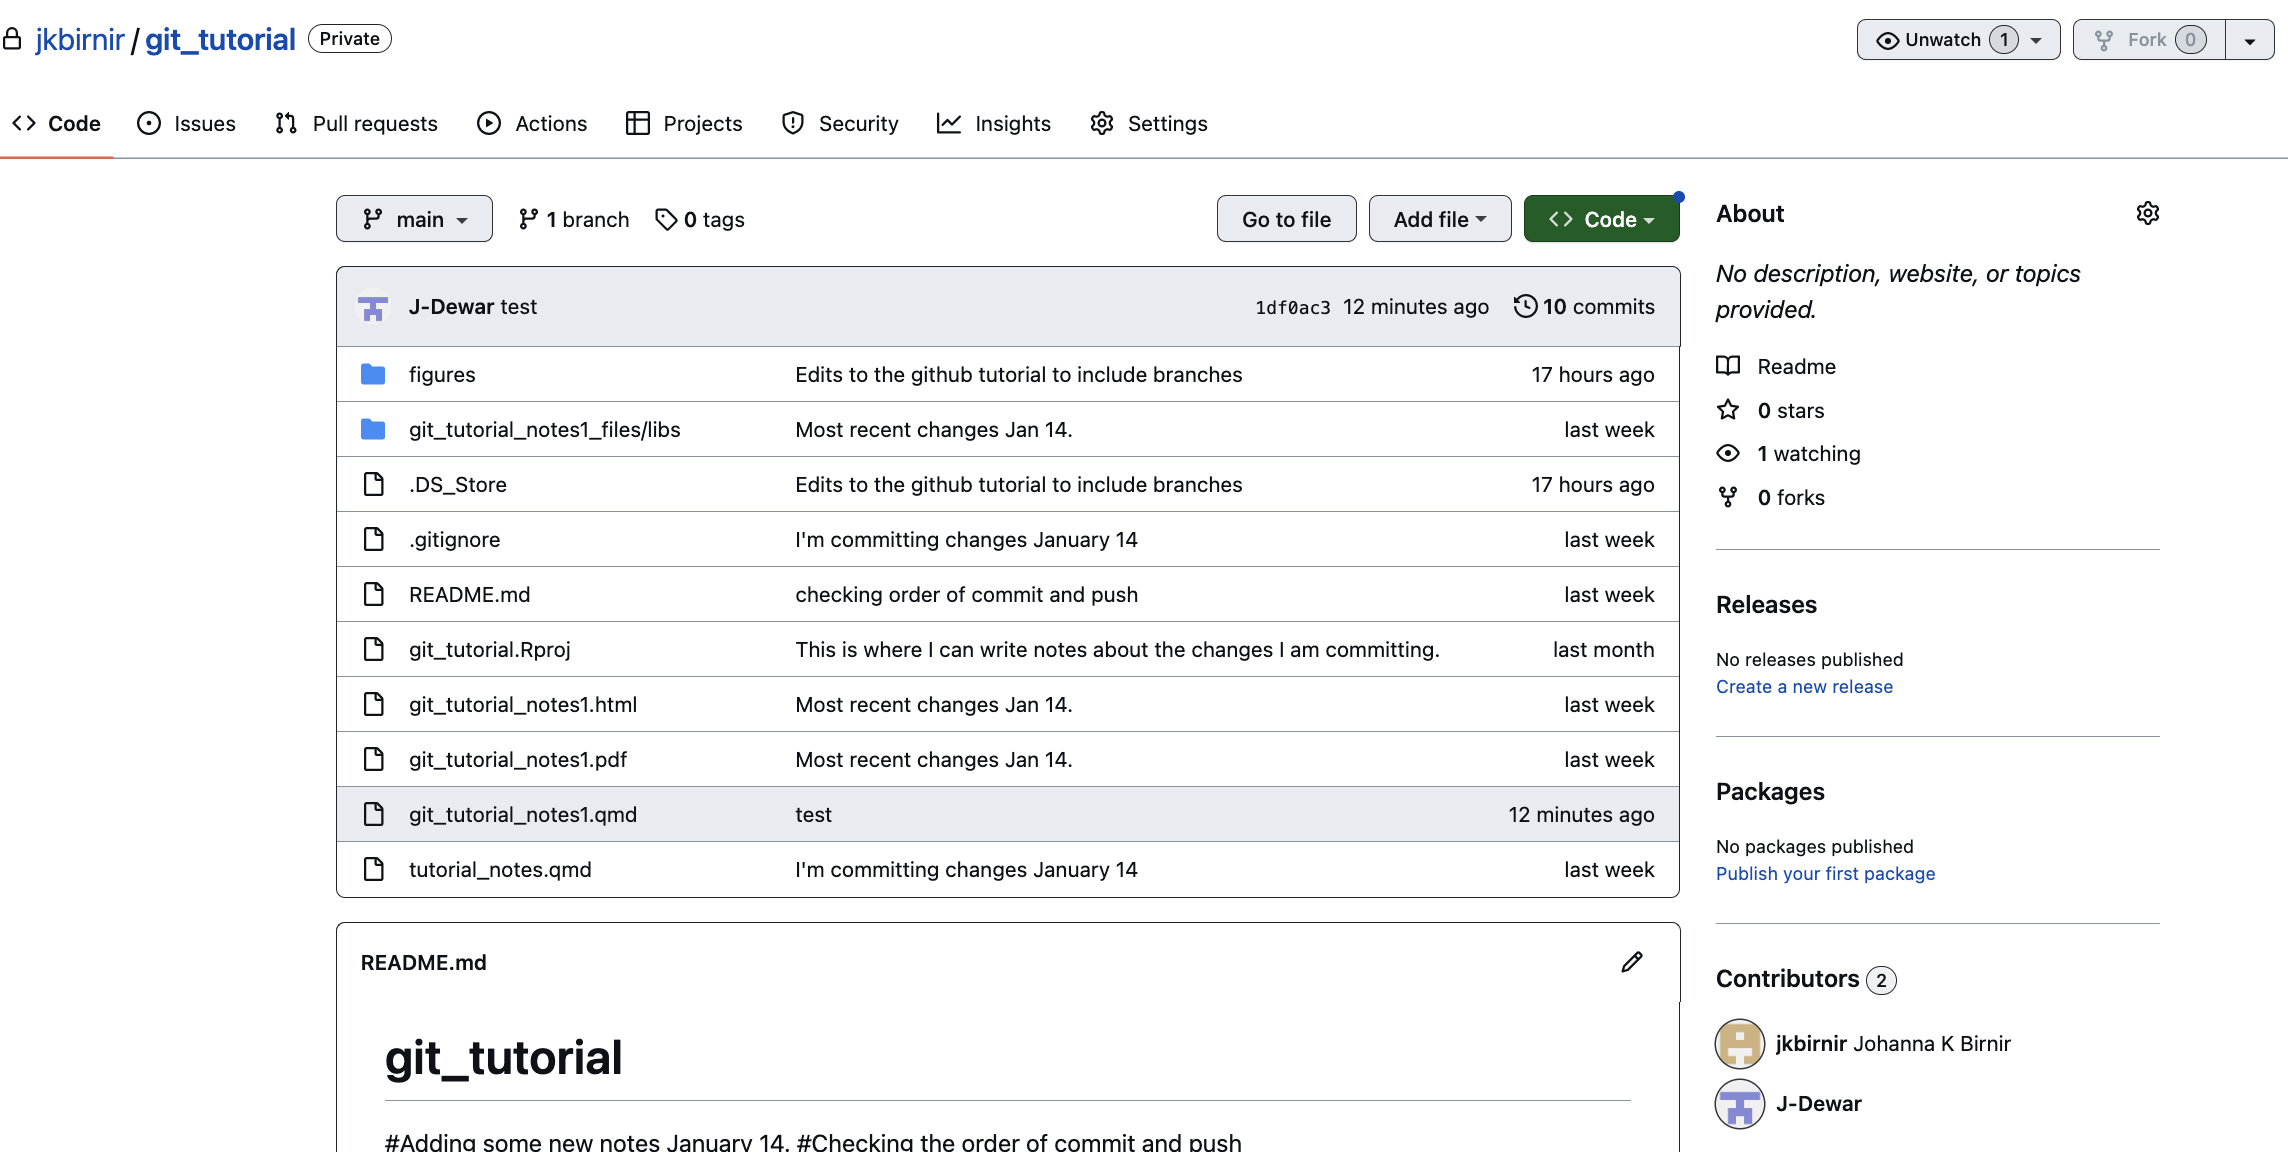
\includegraphics{figures/20.png} There you see who are the collaborators
and when each item was updated. For even more information click on any
of the files (here the qmd file)

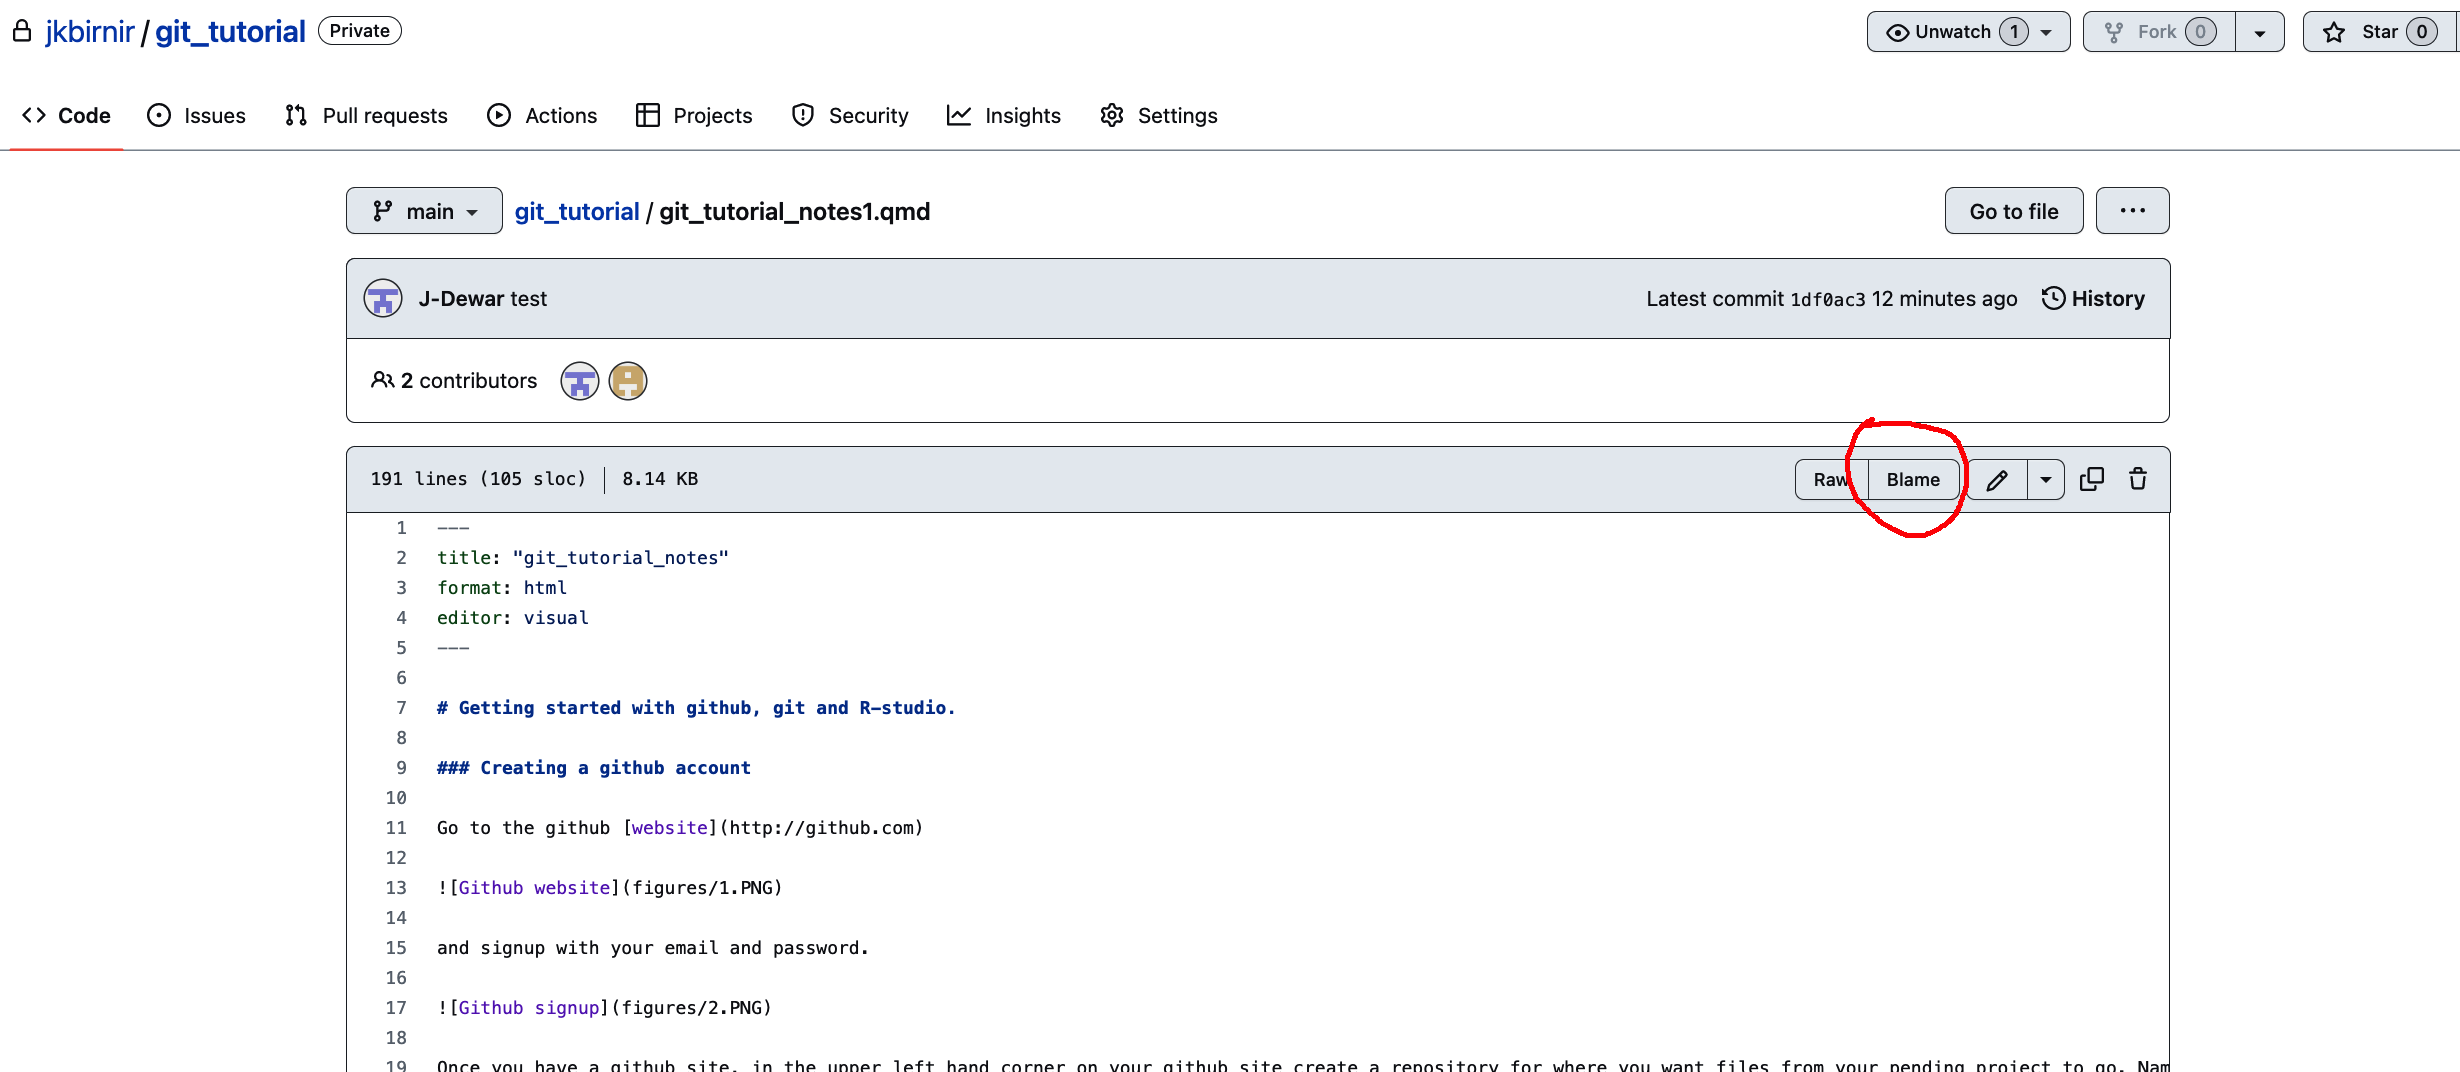
\includegraphics{figures/21.png} Here you see the history of the
development of the project and if you want to see who made what changes
when push the blame button.

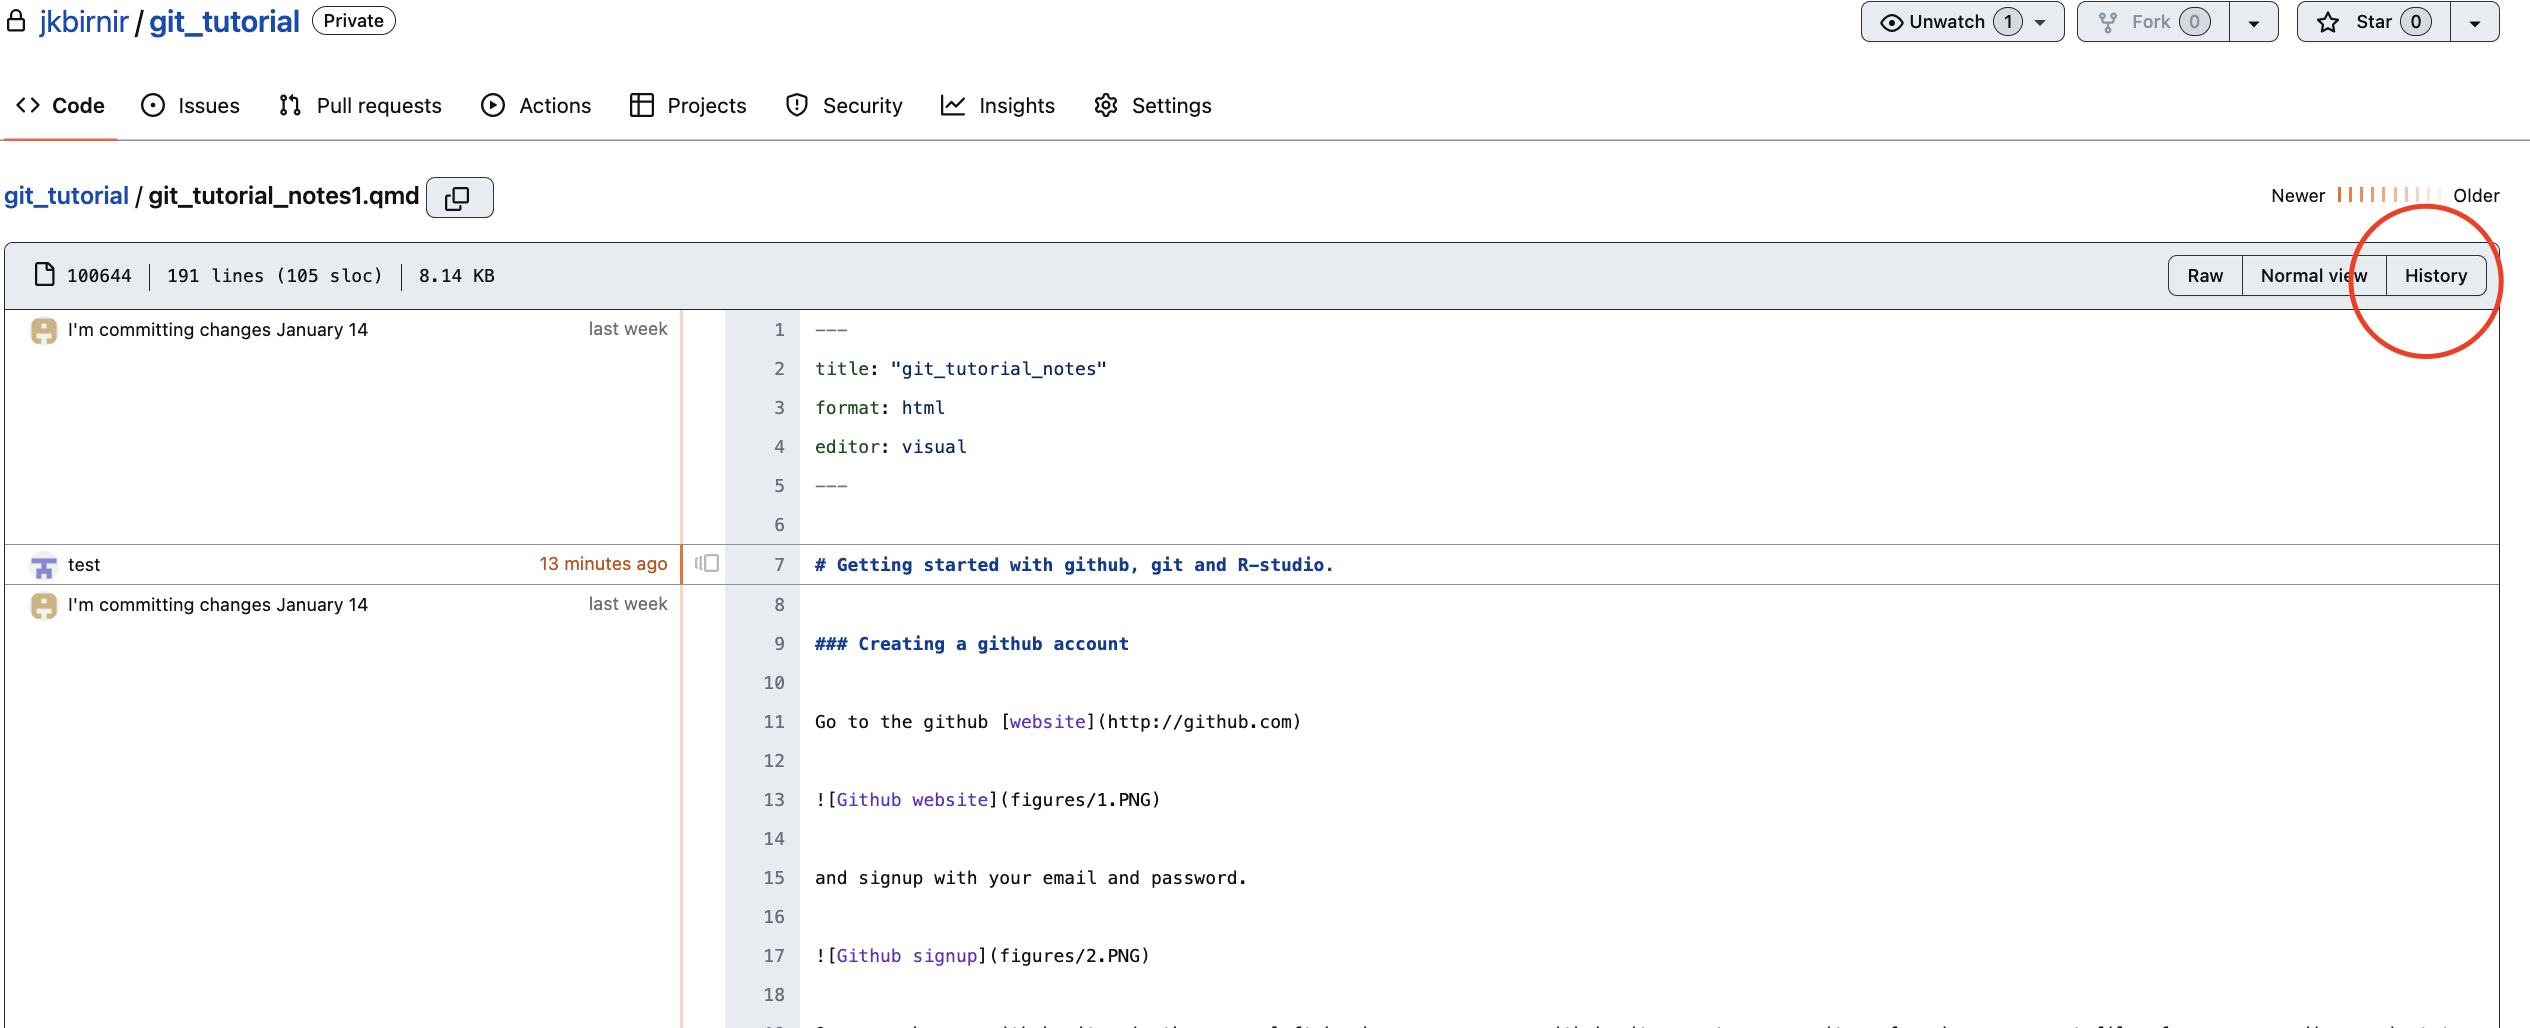
\includegraphics{figures/22.png} The blame allows you to blame whoever -
mostly yourself ;) is responsible for making changes to your project.

If you want more of an overview - then push the history button and you
get a summary of changes:

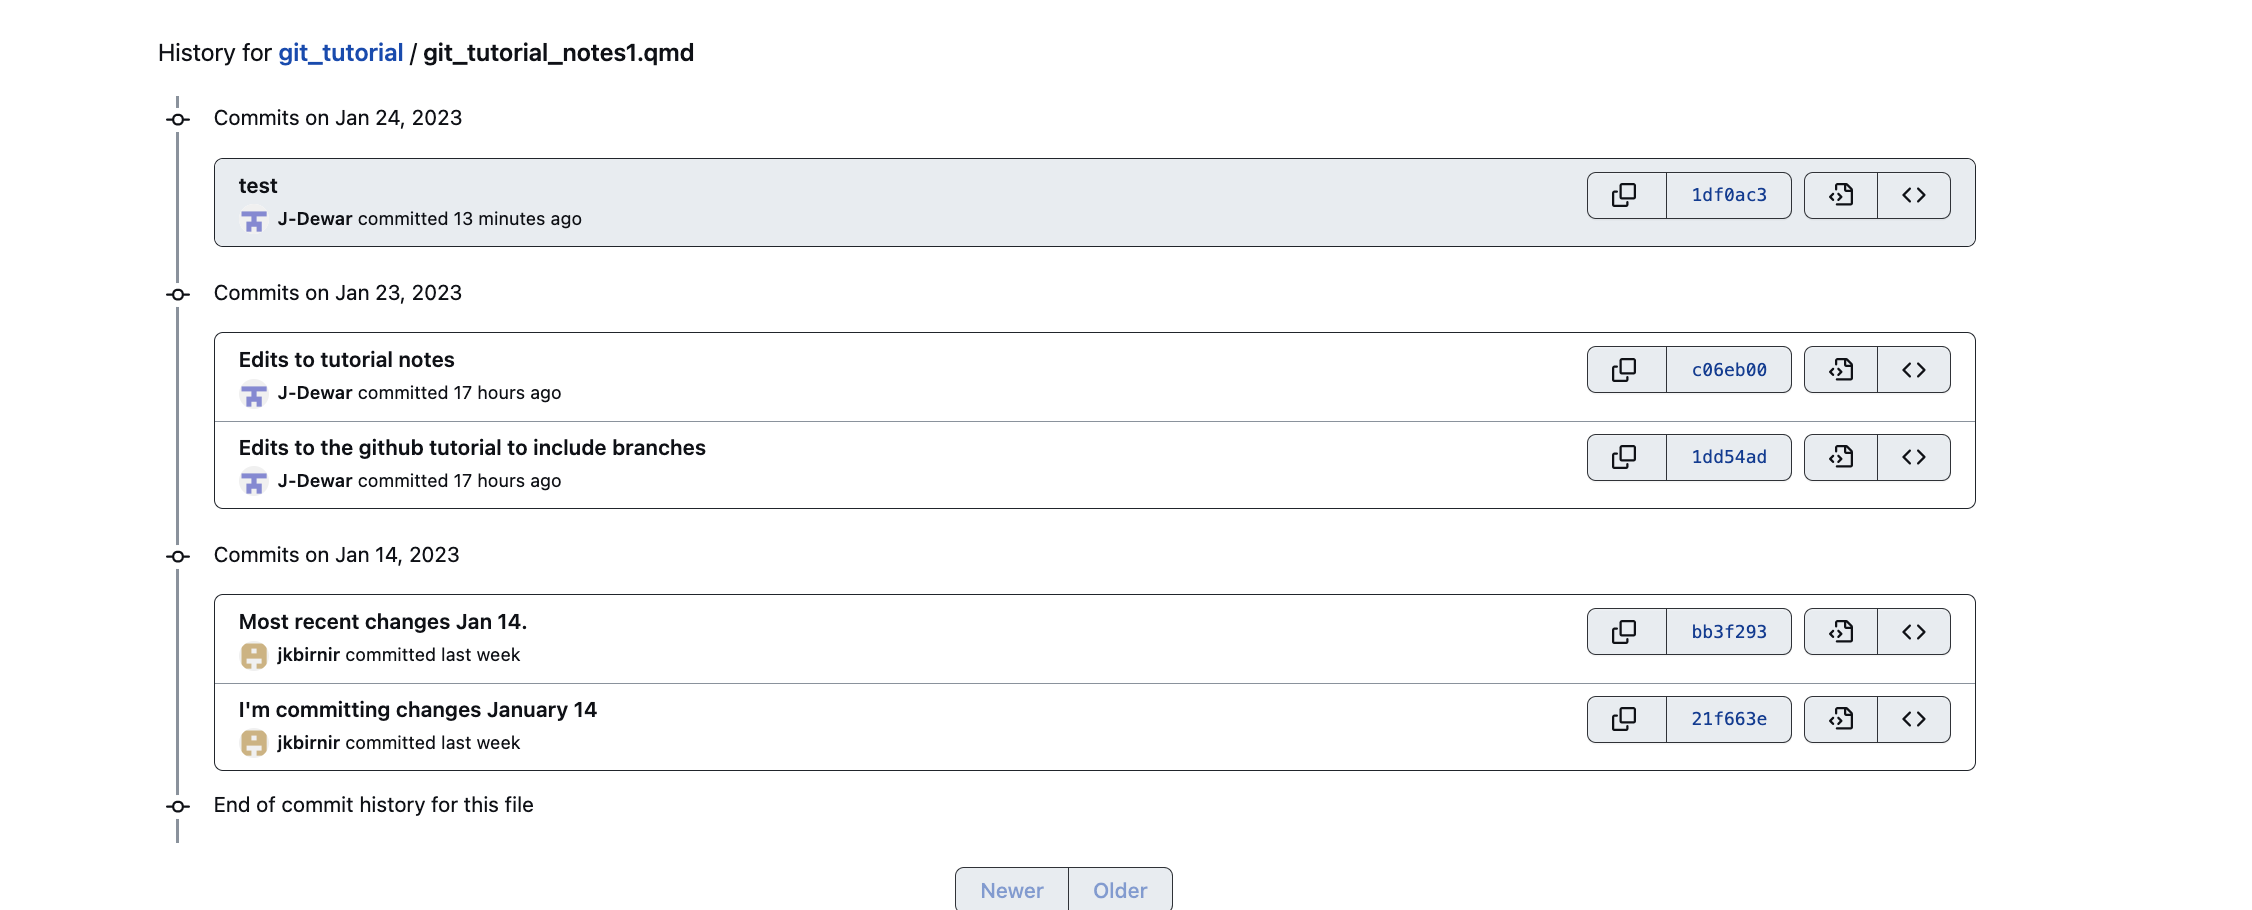
\includegraphics{figures/23.png} In sum this is the workflow when you
and your collaborator are both working on the main project and either
one of you can make changes to the project.

When someone invites you to a project and to work on the main as here:

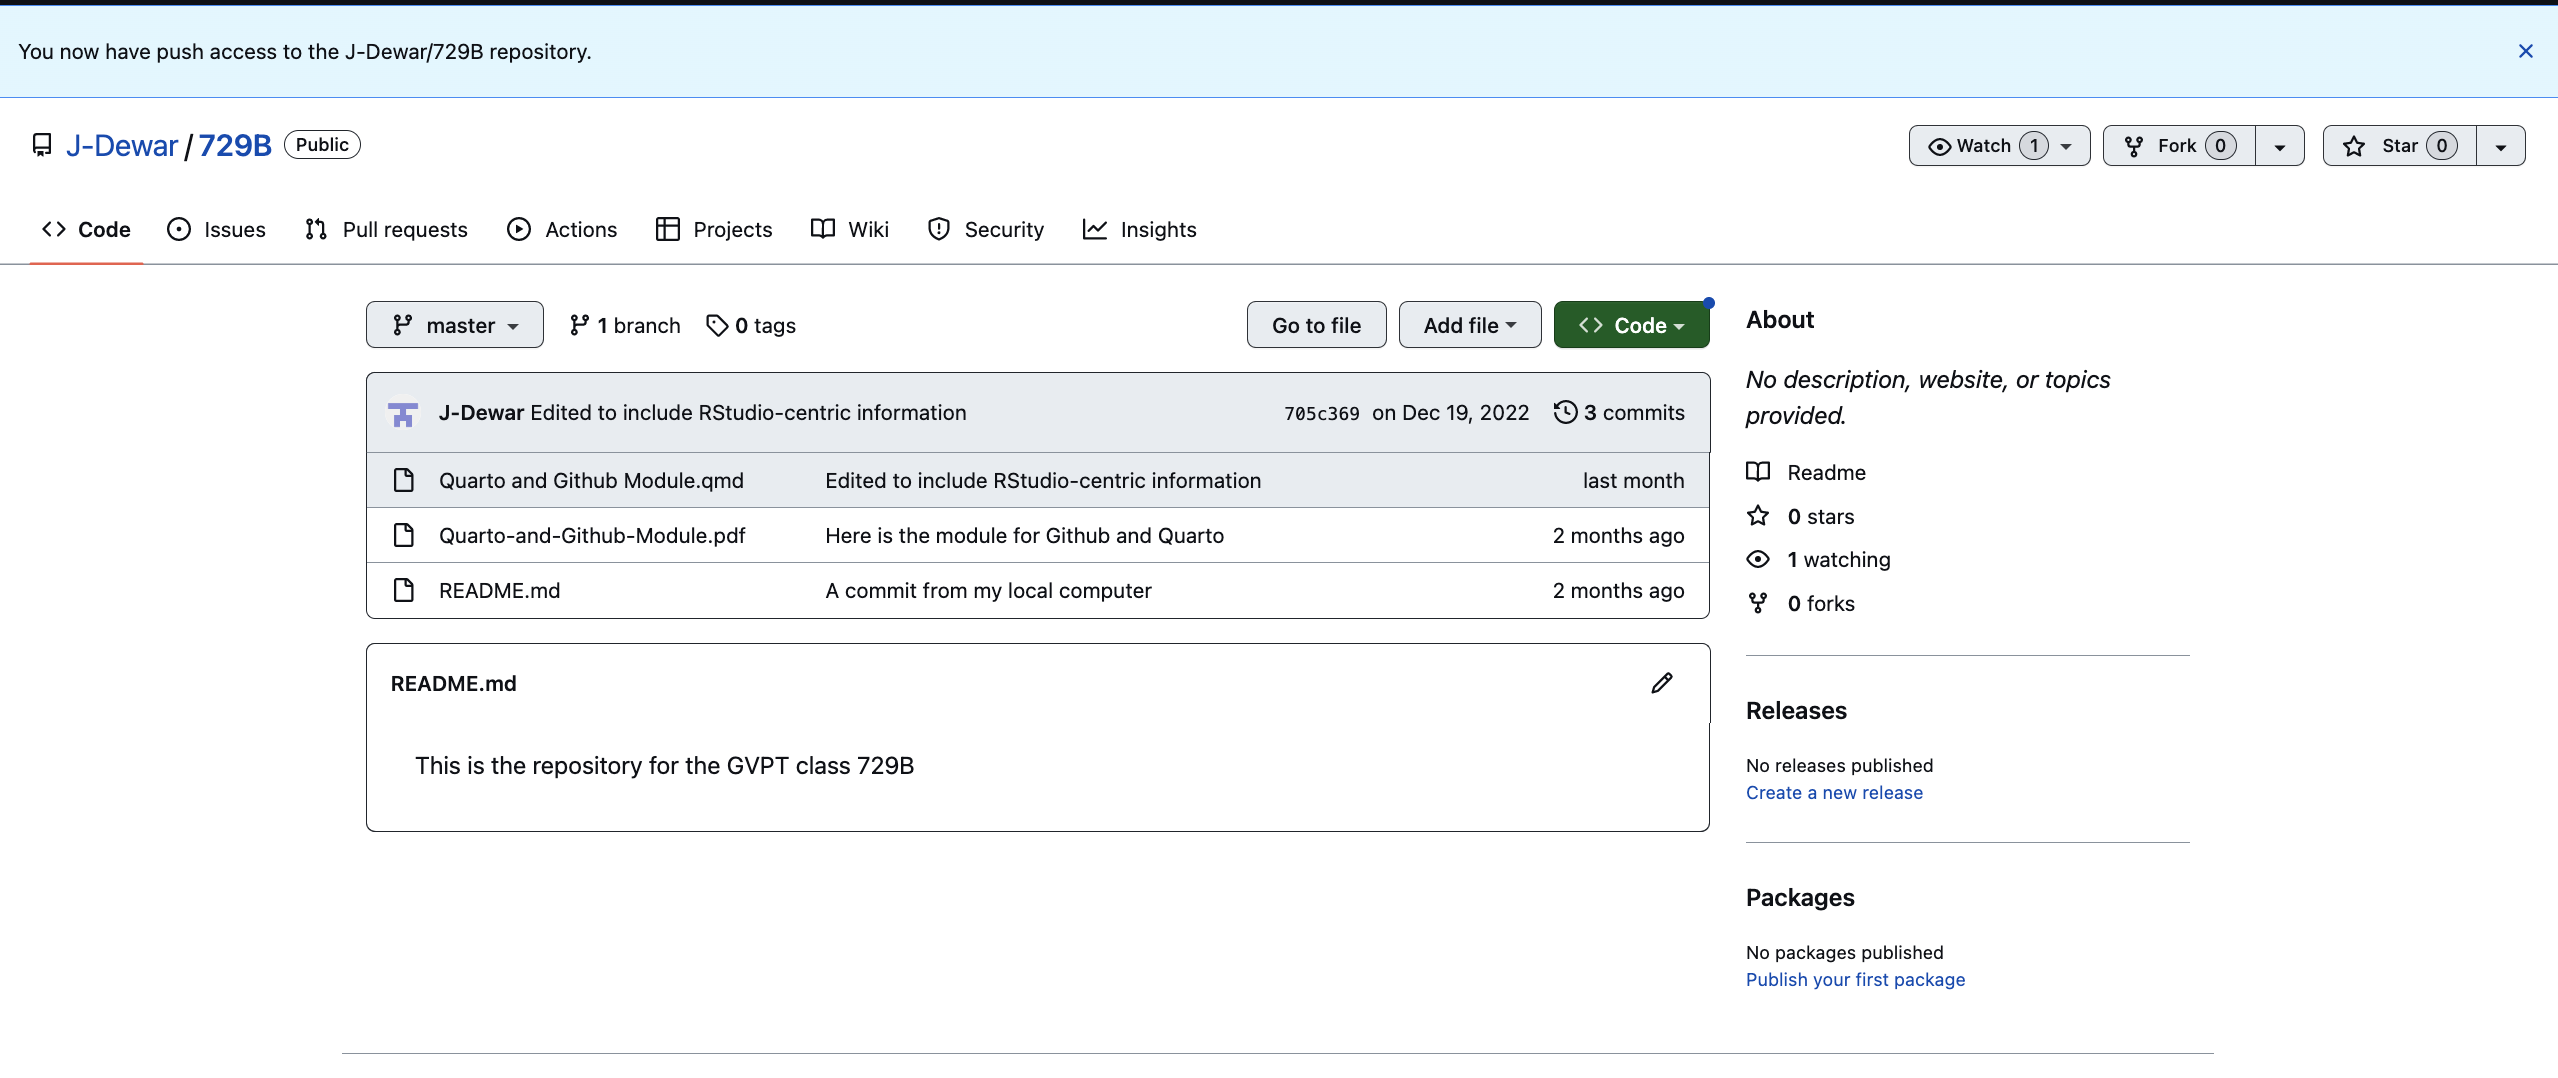
\includegraphics{figures/30.png}

You can open the project locally as you would any other version control
project (see earlier steps in the tutorial)

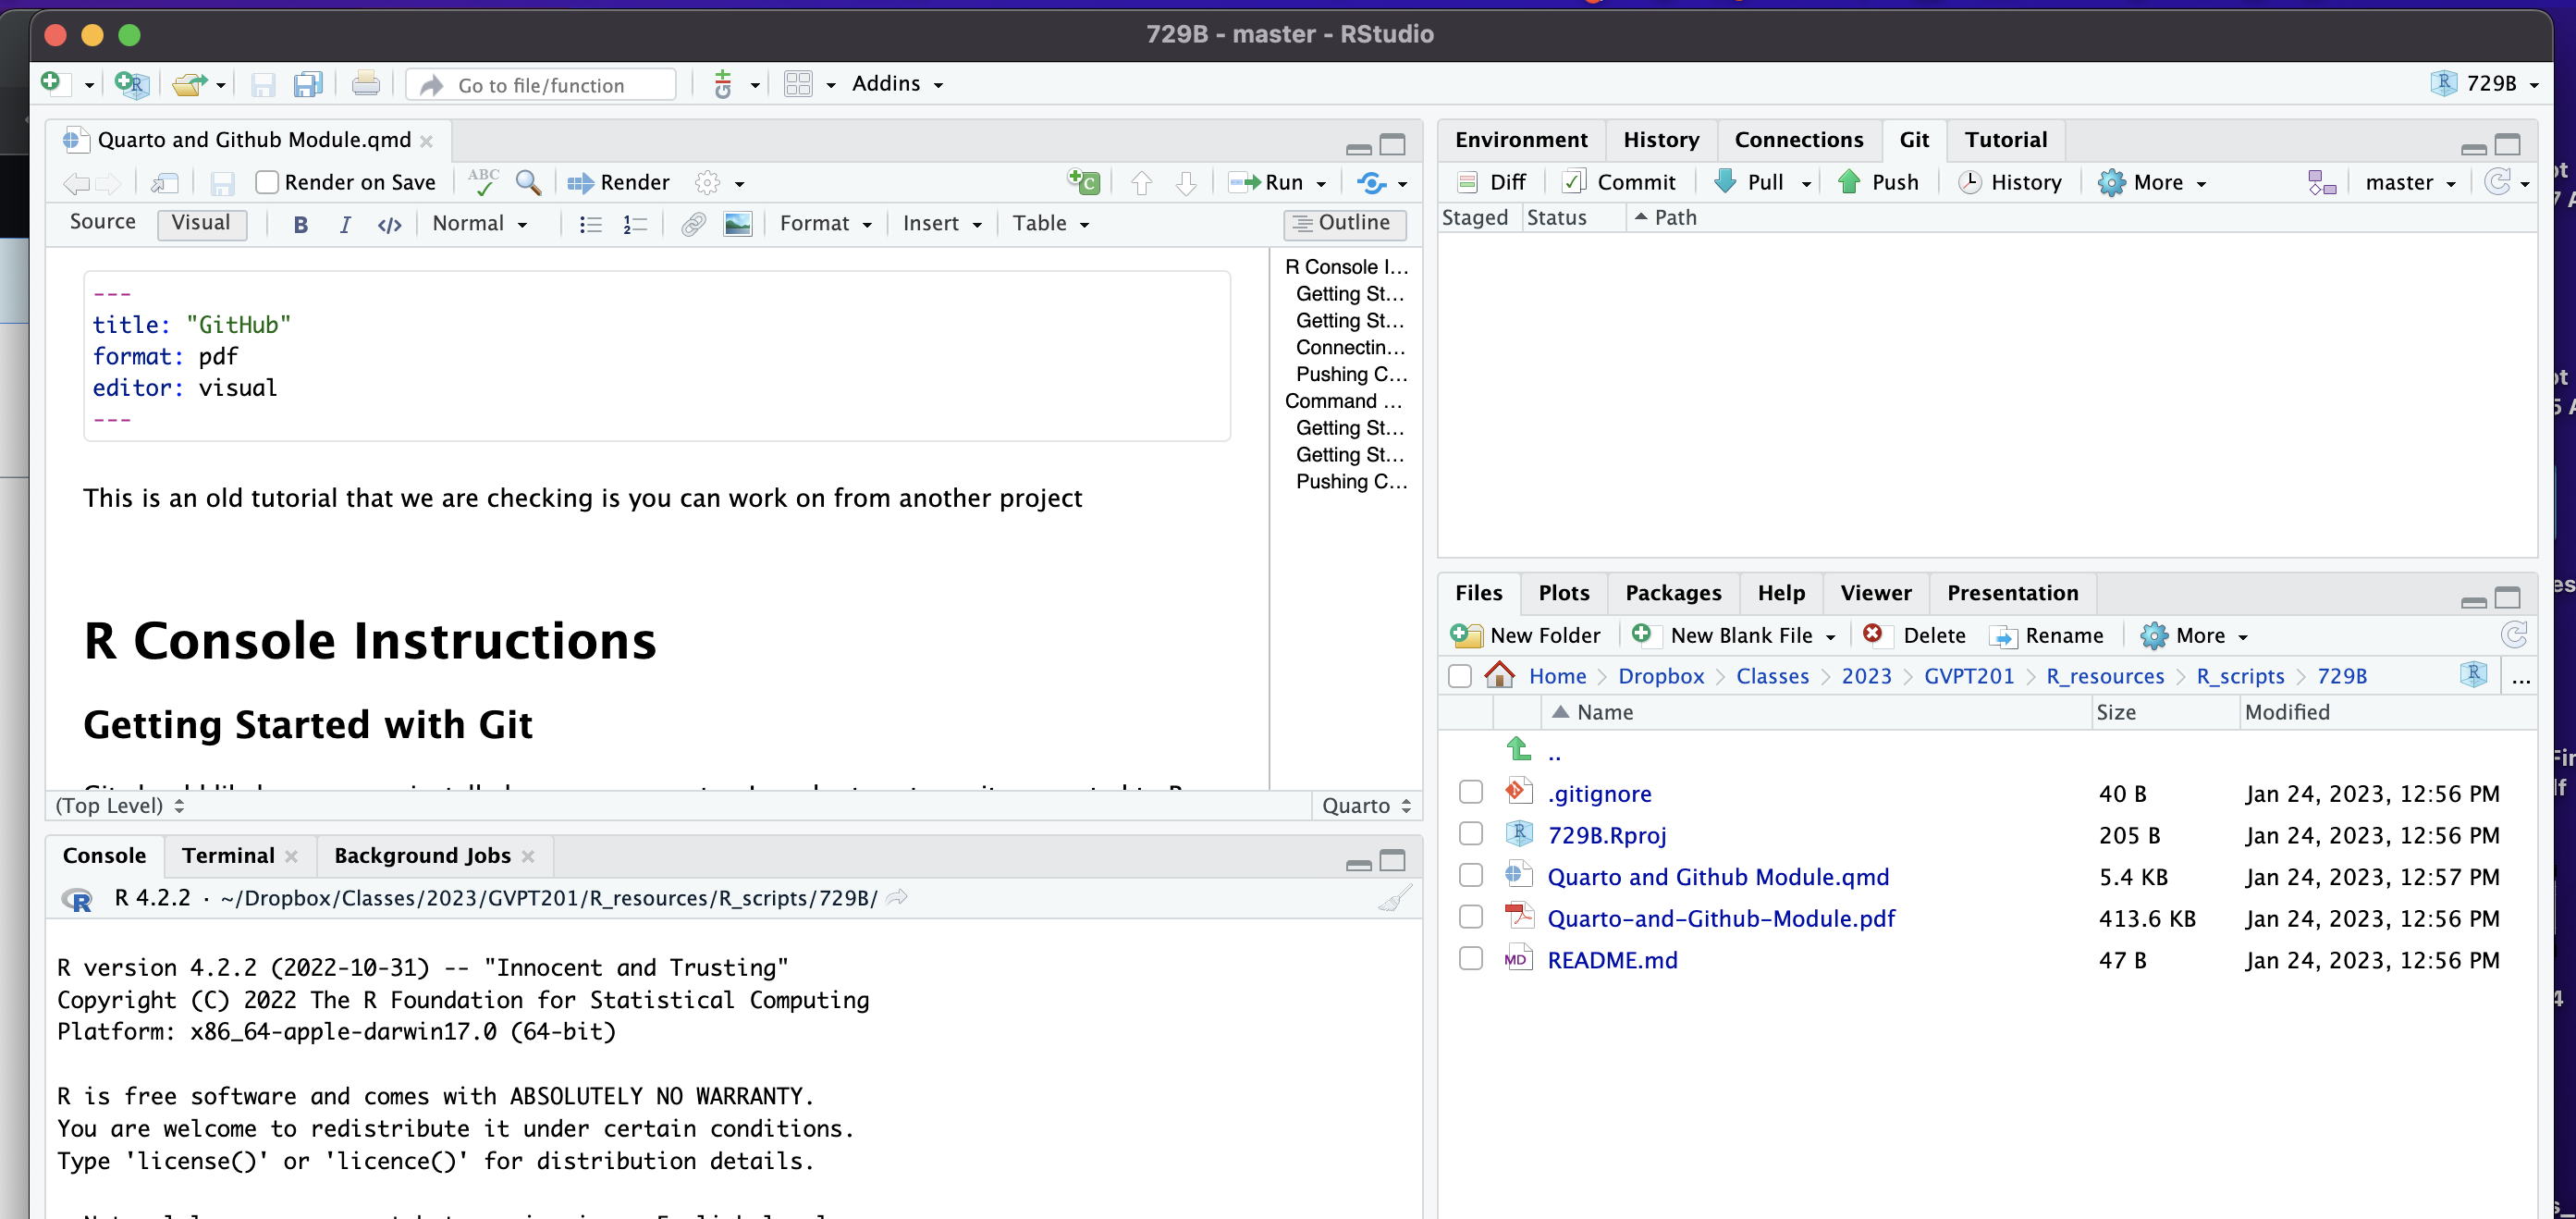
\includegraphics{figures/31.png}

Once you are done changing your files locally - you then go through the
same steps of committing and pushing. Which results in this message
telling you the process was successful.

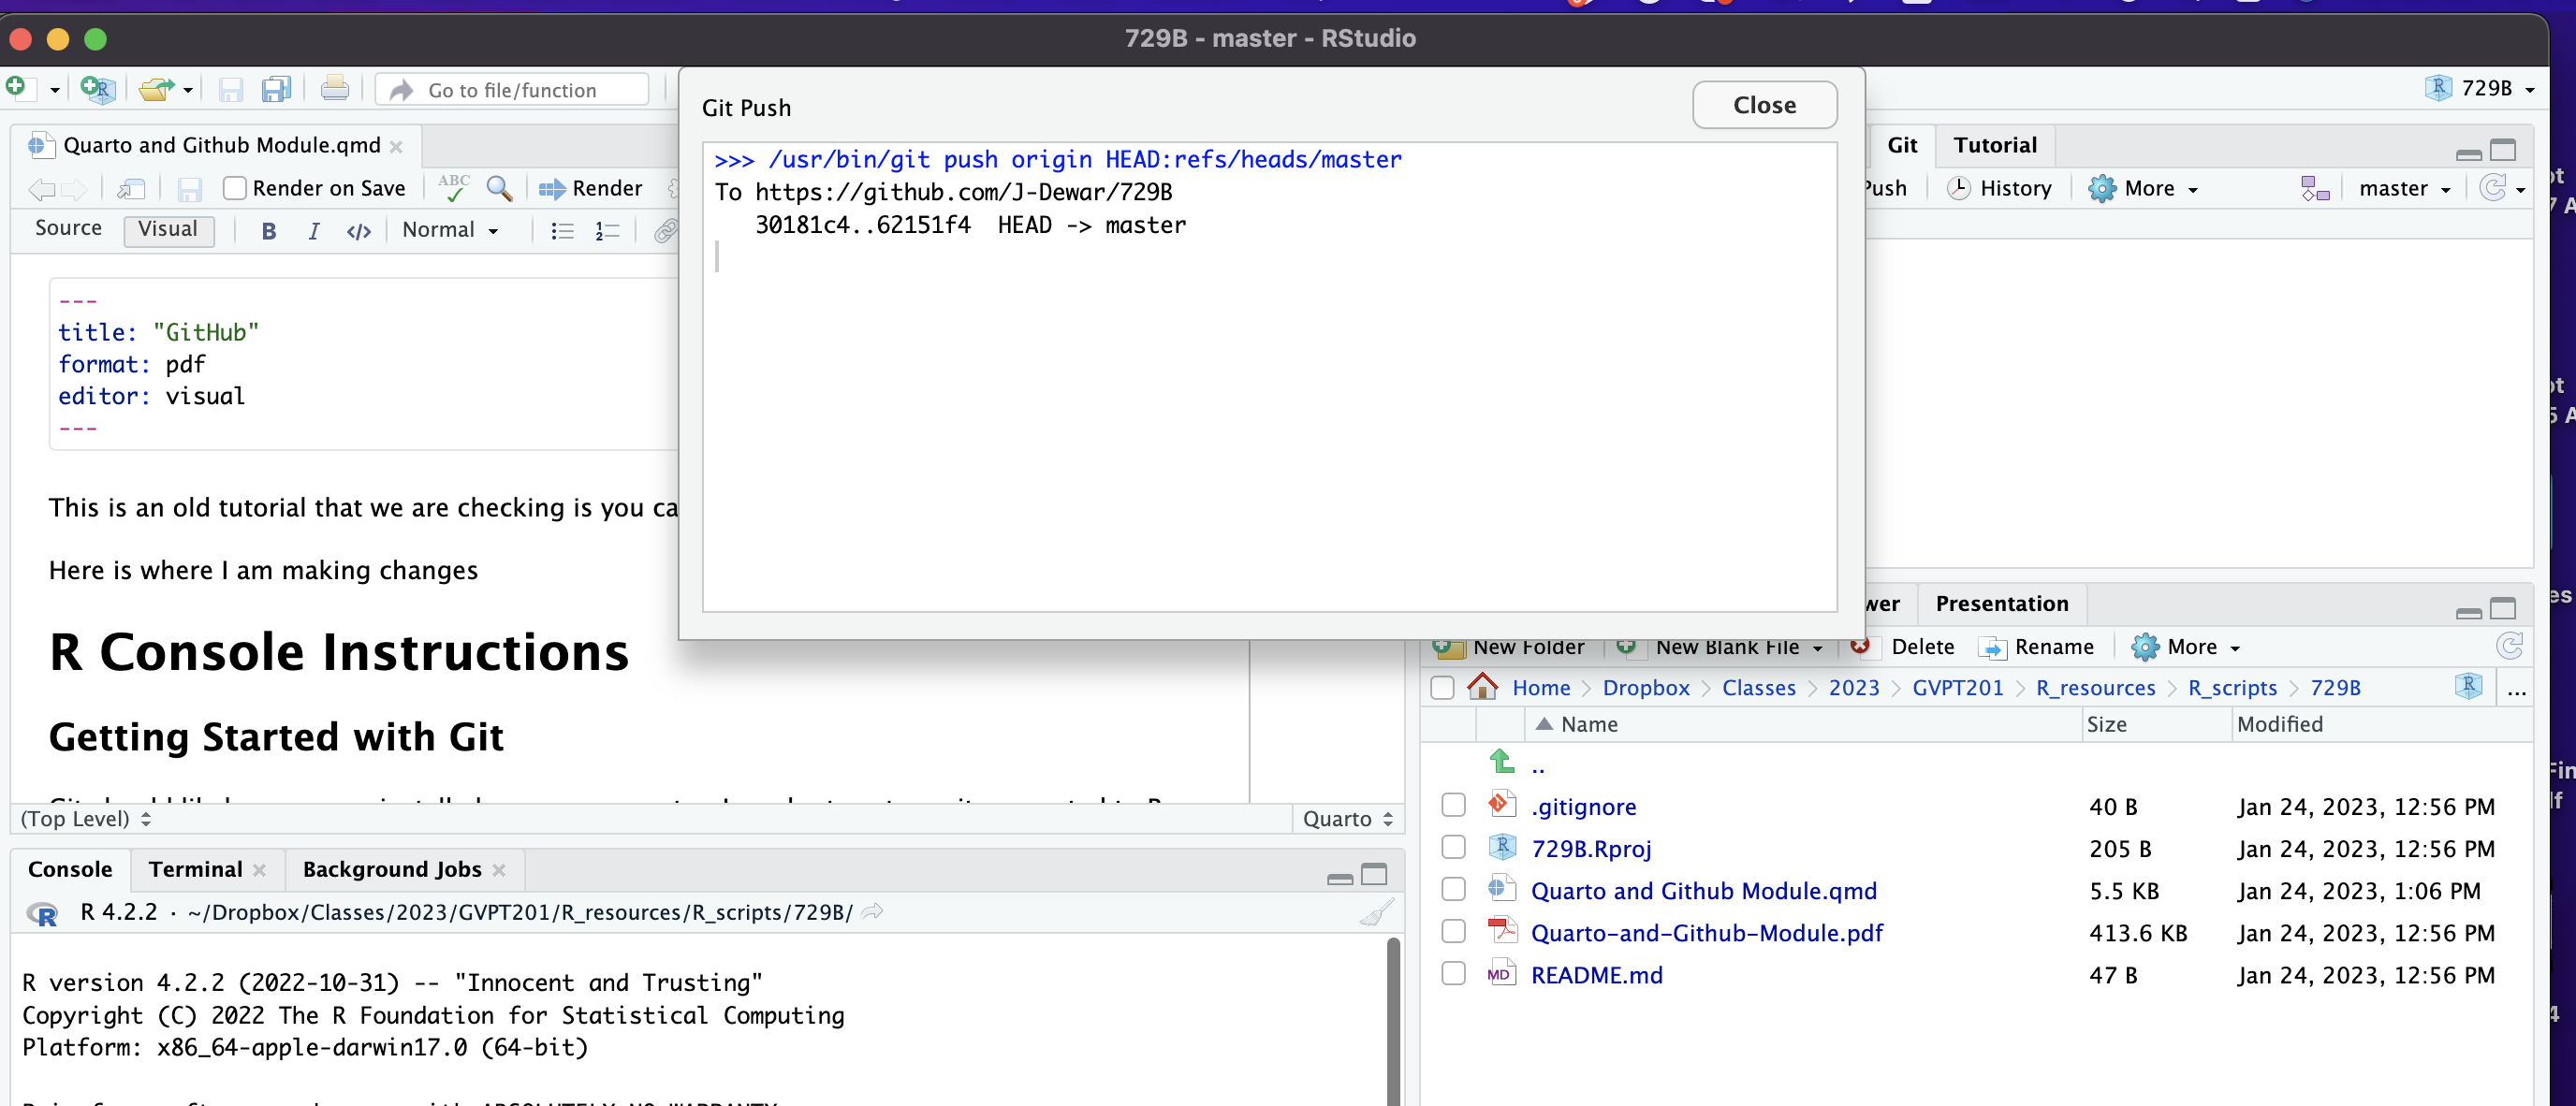
\includegraphics{figures/32.png}

aand your changes will show up in the remote directory on github.

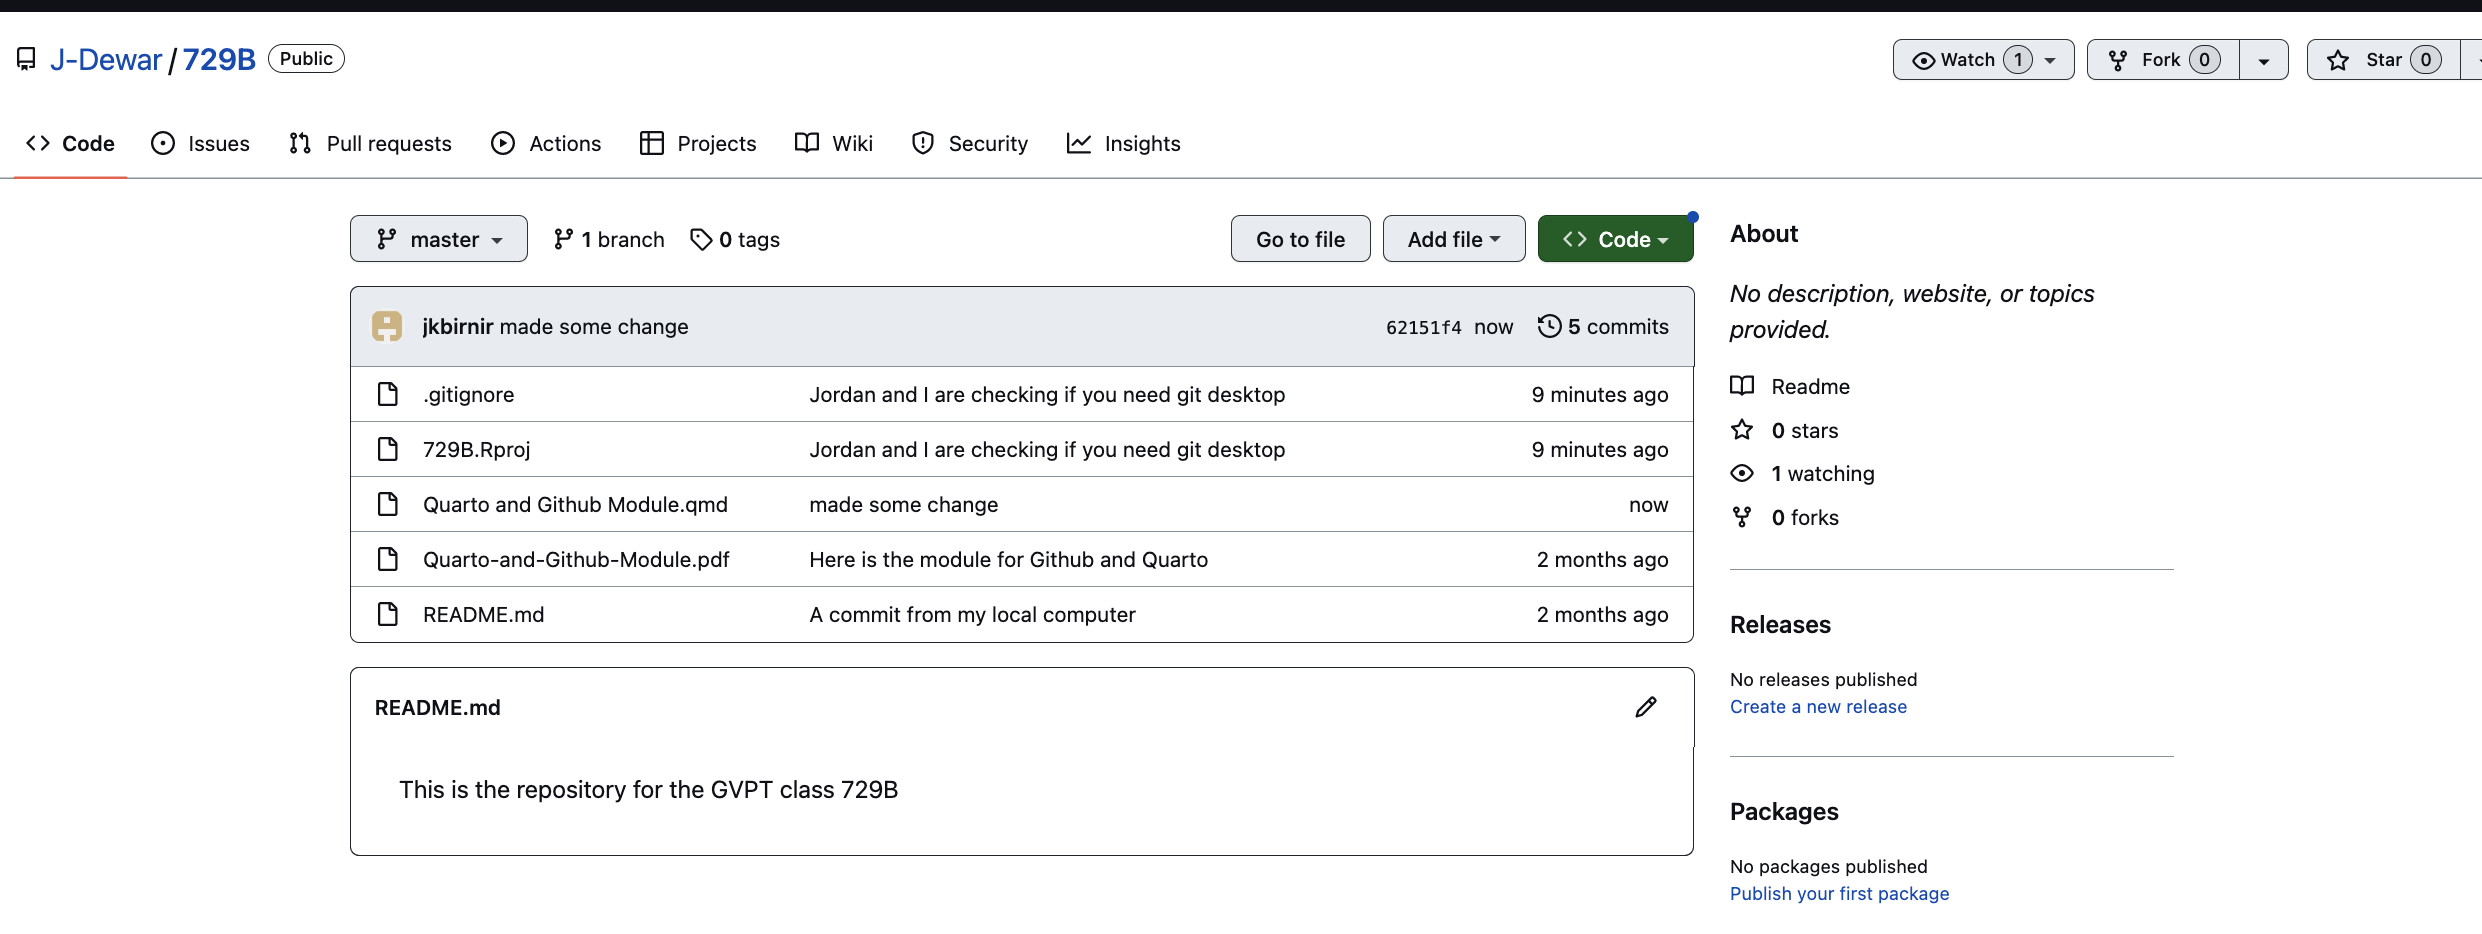
\includegraphics{figures/33.png}

\hypertarget{branches}{%
\subsection{Branches}\label{branches}}

Sometimes you have a hirearchy - when one of you is the lead (author for
example, or if you are working with an RA etc). where you want to review
and approve any changes before they are made. In those cases you work
with branches.

In order to create new branches, go to the `git' tab on your RStudio
console and click `new branch'.

\begin{figure}

{\centering 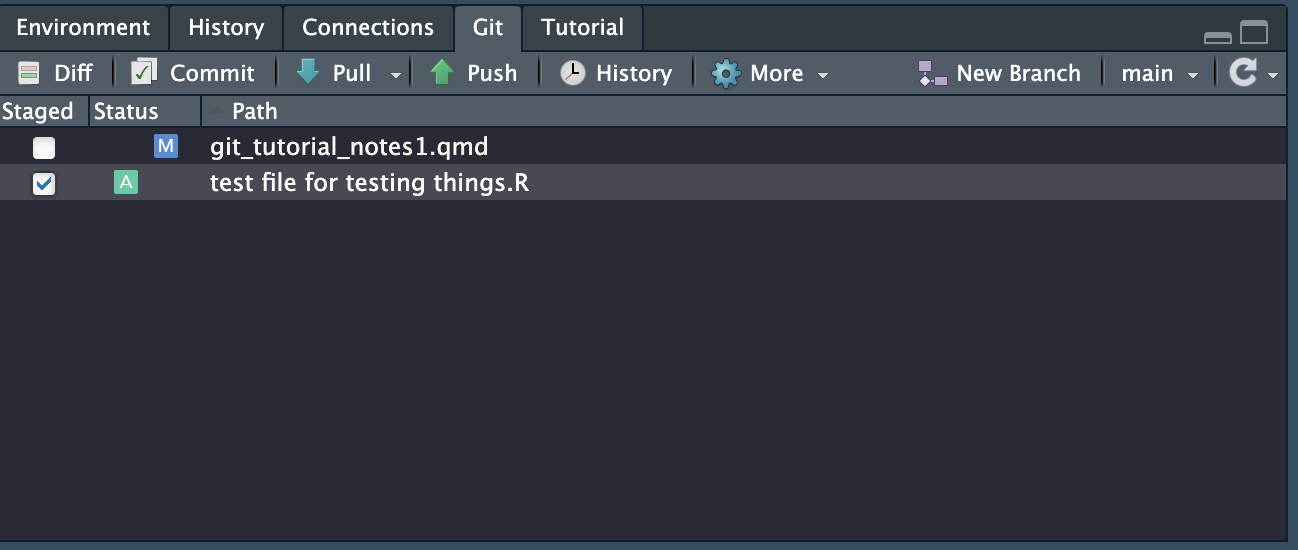
\includegraphics{figures/16.5.png}

}

\caption{Creating a New Branch}

\end{figure}

You can then populate that branch the way you want and ask your
associate to work on that branch only (your associate can also create a
branch to be reviewed later)

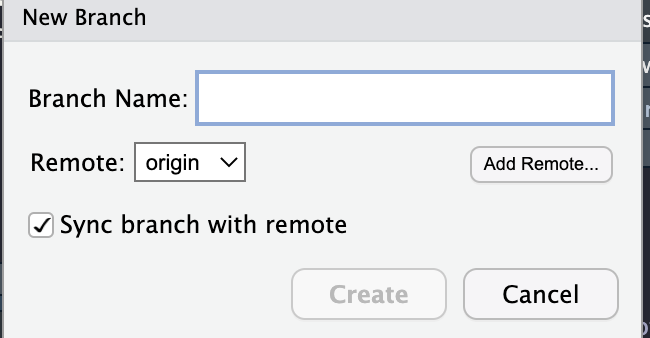
\includegraphics{figures/17.png}

Then click create and you have made the new branch.

You can see your branches like so:

\begin{figure}

{\centering 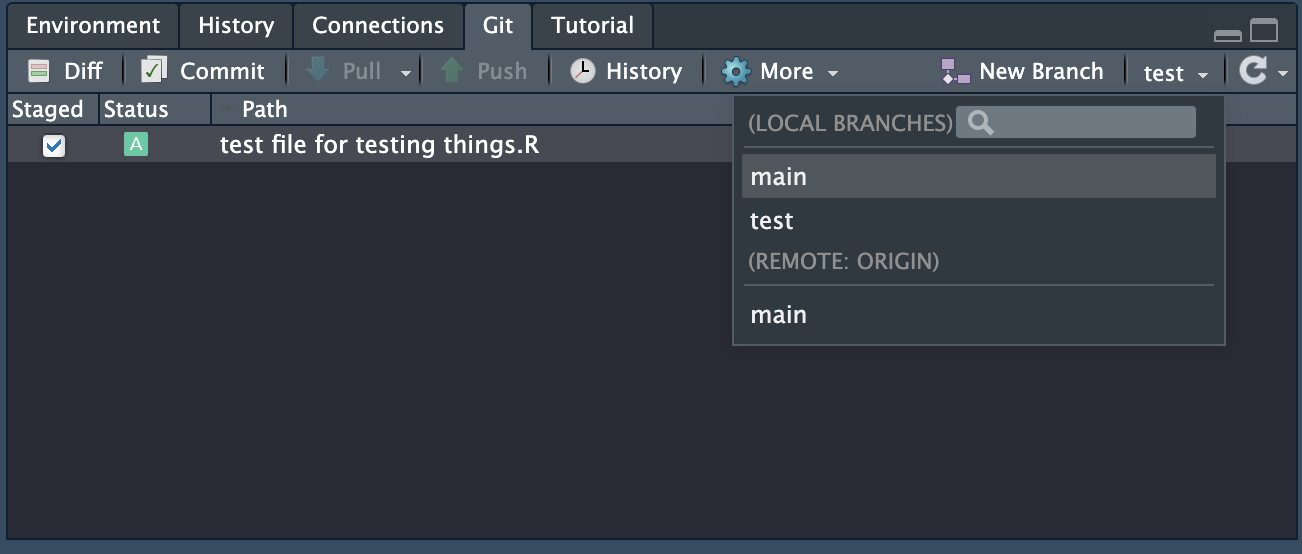
\includegraphics{figures/24.png}

}

\caption{Seeing Branches}

\end{figure}

Then simply create the new branch and you're done.

If you click on the new branch, you will then see this as you switch:

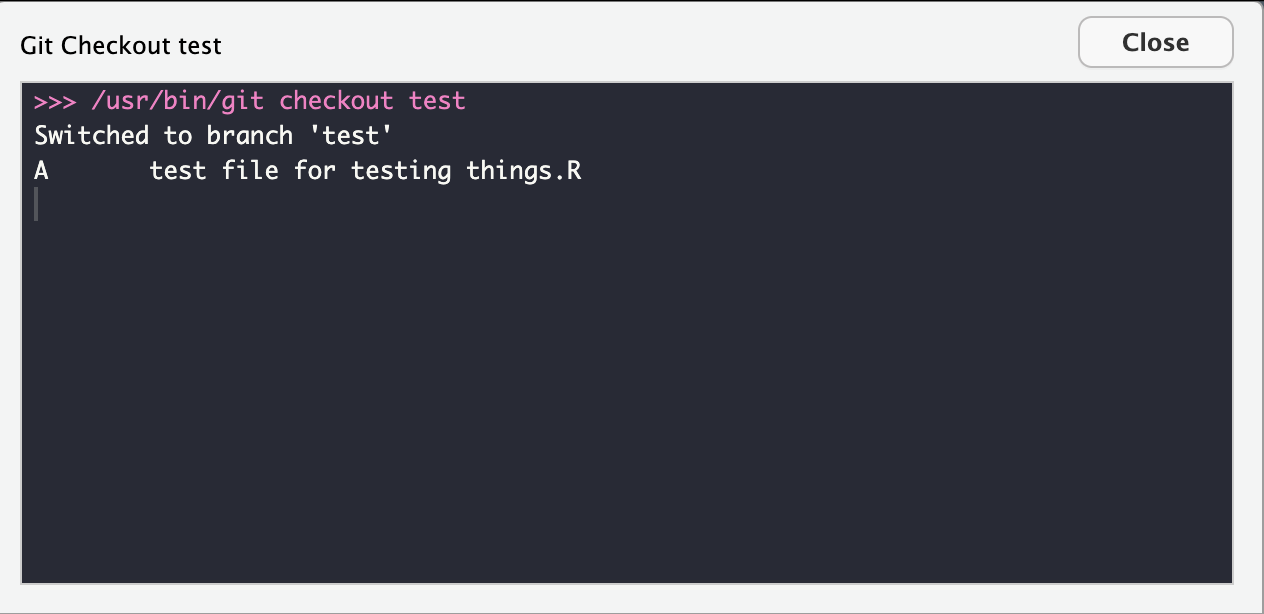
\includegraphics{figures/25.png}

This branch will initially not be published to the repo. You can publish
it via the github website or the github desktop client.

You will then see this on your github page:

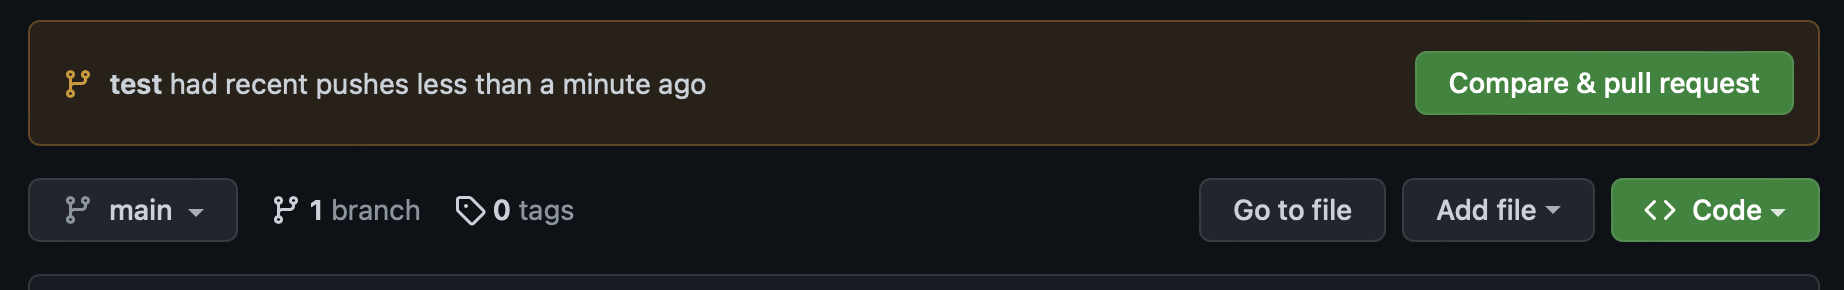
\includegraphics{figures/26.png}

\hypertarget{exercises}{%
\section{Exercises}\label{exercises}}

\hypertarget{start-a-github-project-with-some-documents}{%
\subsubsection{Start a github project with some
documents}\label{start-a-github-project-with-some-documents}}

\hypertarget{invite-your-partner-to-join}{%
\subsubsection{Invite your partner to
join}\label{invite-your-partner-to-join}}

\hypertarget{pull-your-partners-documents}{%
\subsubsection{Pull your partner's
documents,}\label{pull-your-partners-documents}}

\hypertarget{edit-the-documents-commit-the-changes-and-push-changes-to-their-project}{%
\subsubsection{Edit the documents, commit the changes and push changes
to their
project}\label{edit-the-documents-commit-the-changes-and-push-changes-to-their-project}}

\hypertarget{troubleshooting-unintended-branches}{%
\section{Troubleshooting unintended
branches}\label{troubleshooting-unintended-branches}}

If you try to push when you have not pulled changes that your
collaborator has made on a main branch you get the following message:

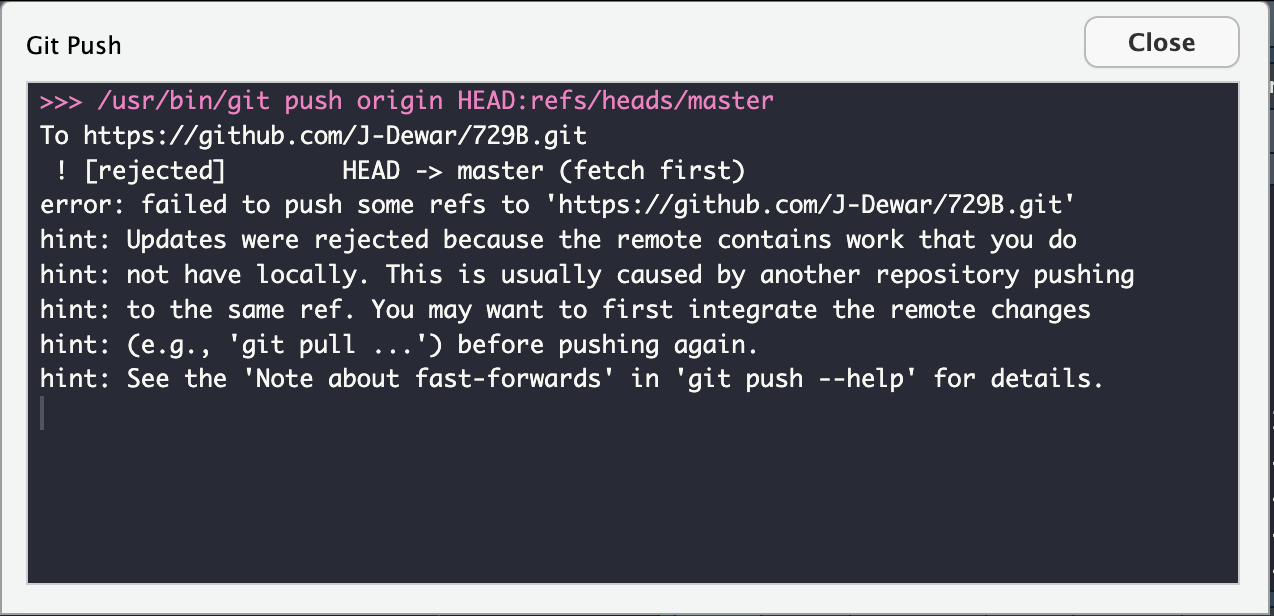
\includegraphics{figures/34.png}

If you try to pull before pushing changes that you have made to
documents that your collaborator has changed you get the following
warning

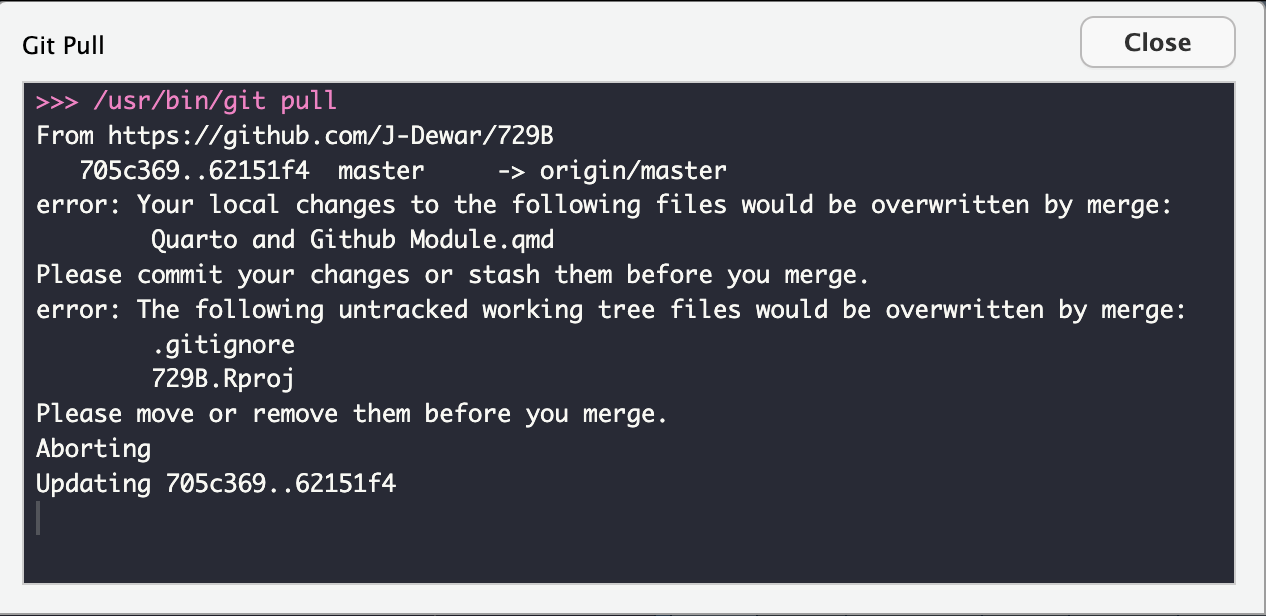
\includegraphics{figures/35.png}

Here the program is creating branches for you so that changes are not
lost. The solution to \#1 is to pull before you start making ay changes
to make sure you are working on the most up to date version. The
solution to \#2 when you both have made changes that need to be
reconciled is to

\begin{enumerate}
\def\labelenumi{\alph{enumi})}
\tightlist
\item
  Committ your local changes then you receive the following message:
\end{enumerate}

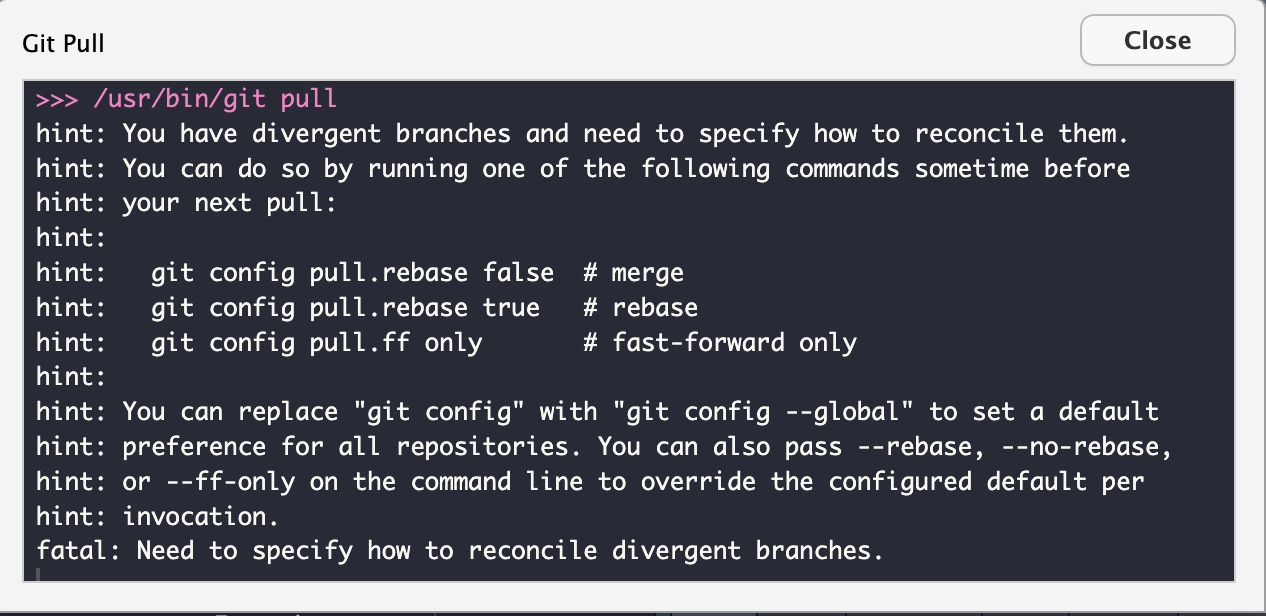
\includegraphics{figures/36.png}

then you pick from the options merge rebase and fast-forward

for a detailed explanation of the differences between the different
options see for example this
\href{https://frontend.turing.edu/lessons/module-3/merge-vs-rebase.html?ads_cmpid=6451354298\&ads_adid=76255849919\&ads_matchtype=\&ads_network=g\&ads_creative=517671727591\&utm_term=\&ads_targetid=dsa-19959388920\&utm_campaign=\&utm_source=adwords\&utm_medium=ppc\&ttv=2\&gclid=CjwKCAiAoL6eBhA3EiwAXDom5hB7rNI86O5HQq3UFkG9tY7t8uBDicj5fL9lc9K_JCyjvZYKz-Wm-RoC97kQAvD_BwE}{website}

To employ the merge solution go to terminal and write:

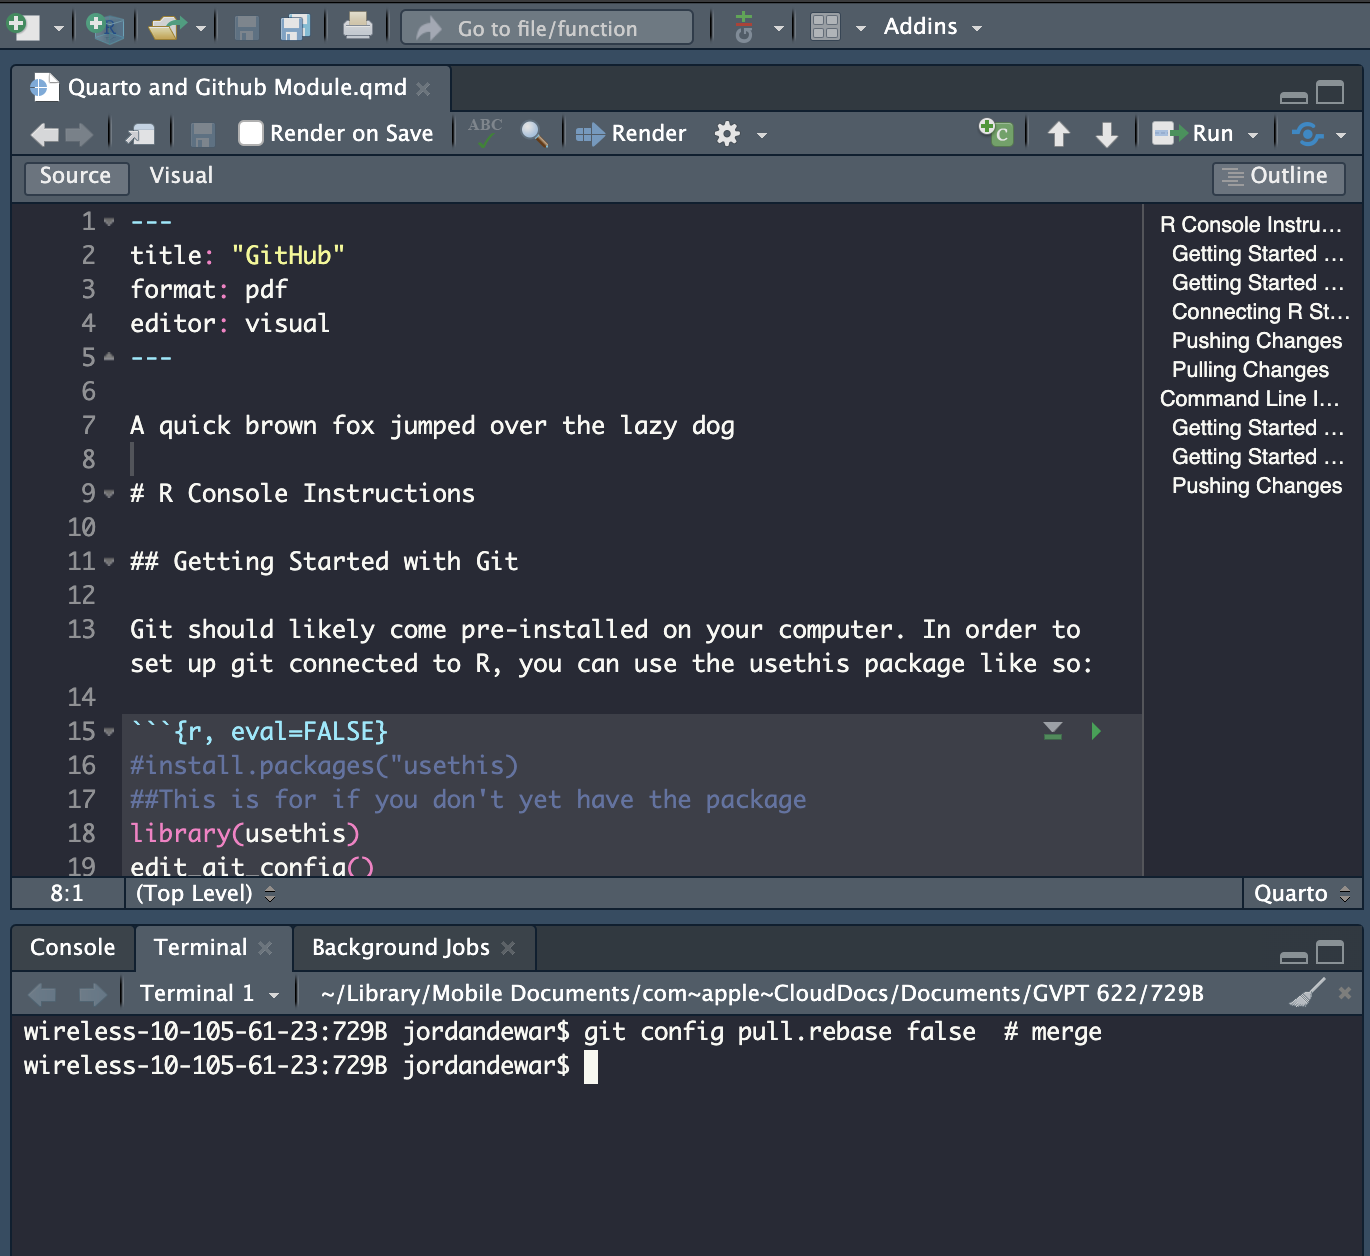
\includegraphics{figures/37.png}

then you can pull the document. Once you pull the document you can
scroll through and see where your merger conflict occurred.

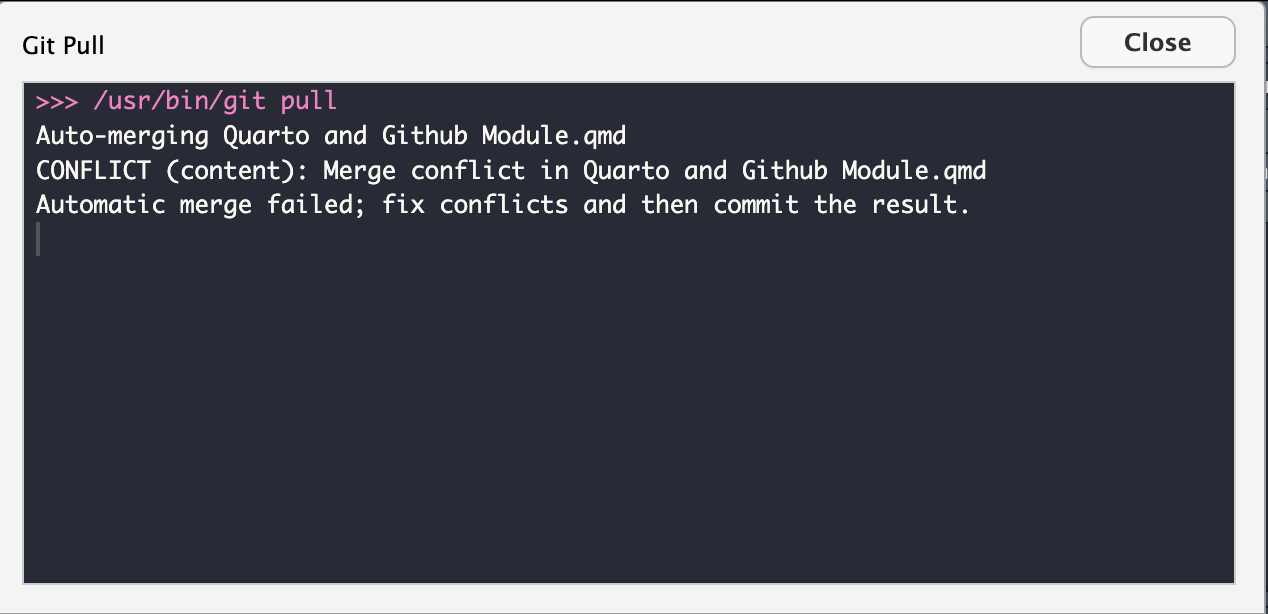
\includegraphics{figures/38.png}

You then have to resolve this conflict save and now you can push.

\hypertarget{good-git-hygene}{%
\section{Good git hygene}\label{good-git-hygene}}

You can look to this
\href{https://betterprogramming.pub/six-rules-for-good-git-hygiene-5006cf9e9e2}{article}
for other useful information for keeping good Git hygiene when
collaborating.

Briefly the first four rules of thumb are:

\hypertarget{always-pull-before-a-push}{%
\subsubsection{\texorpdfstring{\textbf{Always Pull Before a
Push}}{Always Pull Before a Push}}\label{always-pull-before-a-push}}

\hypertarget{pull-frequently}{%
\paragraph{\texorpdfstring{\textbf{Pull
frequently}}{Pull frequently}}\label{pull-frequently}}

\hypertarget{push-infrequently}{%
\paragraph{\texorpdfstring{\textbf{Push
infrequently}}{Push infrequently}}\label{push-infrequently}}

\hypertarget{commit-frequently}{%
\paragraph{\texorpdfstring{\textbf{Commit
Frequently}}{Commit Frequently}}\label{commit-frequently}}

Additionally the
\href{https://betterprogramming.pub/six-rules-for-good-git-hygiene-5006cf9e9e2}{article}
discusses optimal git branch for working together.

\hypertarget{merge-forward-frequently}{%
\paragraph{\texorpdfstring{\textbf{Merge ``forward''
frequently}}{Merge ``forward'' frequently}}\label{merge-forward-frequently}}

\hypertarget{create-pull-requests-infrequently}{%
\paragraph{\texorpdfstring{\textbf{Create Pull Requests
Infrequently}}{Create Pull Requests Infrequently}}\label{create-pull-requests-infrequently}}

To better understand these

\hypertarget{associating-existing-r-studio-projects-with-git}{%
\section{Associating existing r studio projects with
git}\label{associating-existing-r-studio-projects-with-git}}

In order to associate an existing RStudio project with Git you will need
to create a Git repository as described above and then follow the steps
below.

\begin{verbatim}
v Setting active project to '/Users/hannahbirnir/Dropbox/Classes/2023/729B/
Github/Git_tutorial/git_tutorial'
\end{verbatim}

You will then get a prompt asking if you want to commit the files you've
already created to your repo. Select yes (option 1). You should then
also see the git tab.

\begin{verbatim}
* Call `gitcreds::gitcreds_set()` to register this token in the local Git credential store
  It is also a great idea to store this token in any password-management software that you use
* Open URL 'https://github.com/settings/tokens/new?scopes=repo,user,gist,workflow&description=DESCRIBE THE TOKEN\'S USE CASE'
\end{verbatim}

You will then get a number of options to select about what your token
use case will be. This will be project-dependent.

You can learn more about the selections
{[}here{]}(https://docs.github.com/en/developers/apps/building-oauth-apps/scopes-for-oauth-apps)
to help guide you in your process.

\begin{Shaded}
\begin{Highlighting}[]
\CommentTok{\#library(gitcreds) }
\CommentTok{\#gitcreds\_set()}
\end{Highlighting}
\end{Shaded}

When prompted to enter a token or password, enter the token you just
created. If you have entered one previously, you will be prompted to
choose if you'd like to keep your credentials. If nothing has changed,
select 1 and keep things as they are. If they have, follow the most
applicable selection.

\hypertarget{optional-github-desktop-client}{%
\section{Optional: Github Desktop
Client}\label{optional-github-desktop-client}}

A lot of problems can be resolved by examining the Github desktop
client. It's free and you can download it from the Github website.



\end{document}
